% This is the Reed College LaTeX thesis template. Most of the work 
% for the document class was done by Sam Noble (SN), as well as this
% template. Later comments etc. by Ben Salzberg (BTS). Additional
% restructuring and APA support by Jess Youngberg (JY).
% Your comments and suggestions are more than welcome; please email
% them to cus@reed.edu
%
% See http://web.reed.edu/cis/help/latex.html for help. There are a 
% great bunch of help pages there, with notes on
% getting started, bibtex, etc. Go there and read it if you're not
% already familiar with LaTeX.
%
% Any line that starts with a percent symbol is a comment. 
% They won't show up in the document, and are useful for notes 
% to yourself and explaining commands. 
% Commenting also removes a line from the document; 
% very handy for troubleshooting problems. -BTS

% As far as I know, this follows the requirements laid out in 
% the 2002-2003 Senior Handbook. Ask a librarian to check the 
% document before binding. -SN

%%
%% Preamble
%%
% \documentclass{<something>} must begin each LaTeX document
\documentclass[12pt,twoside]{reedthesis}
% Packages are extensions to the basic LaTeX functions. Whatever you
% want to typeset, there is probably a package out there for it.
% Chemistry (chemtex), screenplays, you name it.
% Check out CTAN to see: http://www.ctan.org/
%%
\usepackage{graphicx,latexsym} 
\usepackage{amssymb,amsthm,amsmath}
\usepackage{longtable,booktabs,setspace} 
\usepackage{tikz}
\usepackage{pifont}
\newcommand{\xmark}{\ding{55}}%
\usepackage{algorithm}
\usepackage{wrapfig}
\usepackage{algpseudocode}
\usepackage{pgfplots,wrapfig}
\usepackage{float}
\floatstyle{boxed} 
\usetikzlibrary{positioning}
\usepackage{chemarr} %% Useful for one reaction arrow, useless if you're not a chem major
\usepackage[hyphens]{url}
\usepackage{rotating}
\usepackage{natbib}
\usepackage{amsmath}
\usepackage{algorithm}
\usepackage{algpseudocode}
% Comment out the natbib line above and uncomment the following two lines to use the new 
% biblatex-chicago style, for Chicago A. Also make some changes at the end where the 
% bibliography is included. 
%\usepackage{biblatex-chicago}
%\bibliography{thesis}

%\usepackage{times} % other fonts are available like times, bookman, charter, palatino

\title{An Expansion of Miss Ratio Curves}
\author{Finn P. Hill}
% The month and year that you submit your FINAL draft TO THE LIBRARY (May or December)
\date{May 2023}
\division{Mathematical and Natural Sciences}
\advisor{Charles McGuffey}
%If you have two advisors for some reason, you can use the following
%\altadvisor{Your Other Advisor}
%%% Remember to use the correct department!
\department{Computer Science}
% if you're writing a thesis in an interdisciplinary major,
% uncomment the line below and change the text as appropriate.
% check the Senior Handbook if unsure.
%\thedivisionof{The Established Interdisciplinary Committee for}
% if you want the approval page to say "Approved for the Committee",
% uncomment the next line
%\approvedforthe{Committee}

\setlength{\parskip}{0pt}
%%
%% End Preamble
%%
%% The fun begins:
\pgfplotsset{compat=1.18} 
\begin{document}

  \maketitle
  \frontmatter % this stuff will be roman-numbered
  \pagestyle{empty} % This removes page numbers from the frontmatter

% Acknowledgements (Acceptable American spelling) are optional
% So are Acknowledgments (proper English spelling)
    \chapter*{Acknowledgements}
	I want to thank Riley Shahar who helped me prove a lot of results and without whom I would not have completed this project. I also want to thank Michael Sarris for sparking my interest in Computer Science. Finally, I would like to thank Charlie McGuffey, who has been the best thesis advisor I could ask for and has helped make this into an actual thesis. I would also like to thank my family, Olivia, and others who have helped get me here today. 

% The preface is optional
% To remove it, comment it out or delete it.
	

    \chapter*{List of Abbreviations}

	\begin{table}[H]
	\centering % You could remove this to move the table to the left
	\begin{tabular}{ll}
		\textbf{LRU}  	&  Least Recently Used \\
		\textbf{SCP}  	&  Sum Cost Priority\\
		\textbf{MRC}  	&  Miss Ratio Curve \\
		\textbf{OPT}  	&  Optimal Algorithm\\
        \textbf{CPU}  	&  Computer Processing Unit\\
	\end{tabular}
	\end{table}
	

    \tableofcontents
    \listoffigures

% The abstract is not required if you're writing a creative thesis (but aren't they all?)
% If your abstract is longer than a page, there may be a formatting issue.
    \chapter*{Abstract}
	One of the ways we seek to improve a computer's overall performance is through Caching. Caching uses levels of memory that are smaller and faster than main memory, allowing data to be retrieved more time-efficiently. To decide what data is stored in these caches, caching algorithms were created. One way to test these algorithms' performance is by generating miss ratio curves (MRC). These curves show how different cache sizes affect the performance of an algorithm on a trace of items. This MRC generation requires lots of computational work, requiring the algorithm to be tested on every cache size. There is a way around this work, which is through the use of Mattson's algorithm. This algorithm is currently limited to the paging model. We expand efficient MRC creation to the cost model. Our work relies on a new algorithm called Sum Cost Priority (SCP). We show that this algorithm performs within $\pm$5\% of an algorithm with proven theoretical properties on $62.3\%$ of generated traces and 82.1\% of traces from Twitter.

 %TODO: punctuation and grammar: the current way to efficiently generated to limited paging model
%TODO: synthetically gnerated traces vs twitter traces seperate out the claims
 
	\chapter*{Dedication}  
    I have kept my promise, 85\% is always enough.
 
  \mainmatter % Here the regular Arabic numbering starts
  \pagestyle{fancyplain} % turns page numbering back on

%The \introduction command is provided as a convenience.
% If you want special chapter formatting, you'll probably want to avoid using it altogether

    \chapter*{Introduction}
         \addcontentsline{toc}{chapter}{Introduction}
	\chaptermark{Introduction}
	\markboth{Introduction}{Introduction}
	% The three lines above are to make sure that the headers are right, that the intro gets included in the table of contents, and that it doesn't get numbered 1 so that chapter one is 1.

% Double spacing: if you want to double space, or one and a half 
% space, uncomment one of the following lines. You can go back to 
% single spacing with the \singlespacing command.
%\onehalfspacing
%\doublespacing

% Create a summary of the background 
%Create a summary of the results 

%Wording could use work. 



How do computers efficiently store data and access it quickly? 


This problem is at the core of caching in computer systems. The issue with fast data retrieval on computers is that the larger the storage, the slower is it to retrieve data from it. So to make computers run faster, computers mimic large and fast storage. They do this by having ever-decreasing size storage levels called caches, which are smaller and faster than main memory. These caches store a subset of the memory that the computer has access to.

There is an inherent challenge with this system, and that is that instead of having one level of memory with all the data, there are now multiple levels that must be searched.


This search starts in the lowest level, which is small and fast, then if the information isn't there must search the next level. This search process continues until the data is found. Every miss causes a further time penalty as each subsequent layer is slower than the last. The way one attempts to minimize these time penalties is with caching algorithms.

An analytical tool that can be used to display these algorithms' performance on sets of requests is called a Miss Ratio Curve (MRC). 
These MRCs are useful because they show how an algorithm performs with different cache sizes on a set of requests. Though one issue with MRCs is that to create these miss ratios for all cache sizes, an algorithm must be run on all these cache sizes. This repeated calculation of miss ratios takes a lot of computational effort. A solution to this large computational work was proposed by Mattson, which then allows for MRCs to be generated in one pass on a trace, but is limited to traces with items having the same size and cost. 



Our work expands this efficient generation of MRCs by making it no longer necessary for items to have the same cost. We do this through the use of an algorithm called Sum Cost Priority (SCP). SCP performs within $\pm$5\% on 65.07\% of traces when compared to a provably well-performing algorithm called Landlord.

In Chapter 1 we focus on what caching is, why it is important in modern systems, and present a model for the problem. In Chapter 2, we show how processor caches function to give a better understanding of hardware caches. In Chapter 3, we explain caching algorithms and how to compare their performance. In Chapter 4, we explain how MRCs are generated efficiently. In Chapter 5 we explain how we expand MRCs with SCP and we analyze the theoretical and real performance of SCP.
\chapter{Background}
\section{What Caching is}



Making computers more efficient and responsive has been a goal of computer researchers and engineers since the inception of Computer Science. One struggle that persists today is the efficient and timely retrieval of data. Since there is no way to make data storage both fast and large, engineers created caching. The idea behind caching is to combine fast, small memory with large, slow memory to mimic memory that is both large and fast.

\begin{figure}[h]
    \centering
    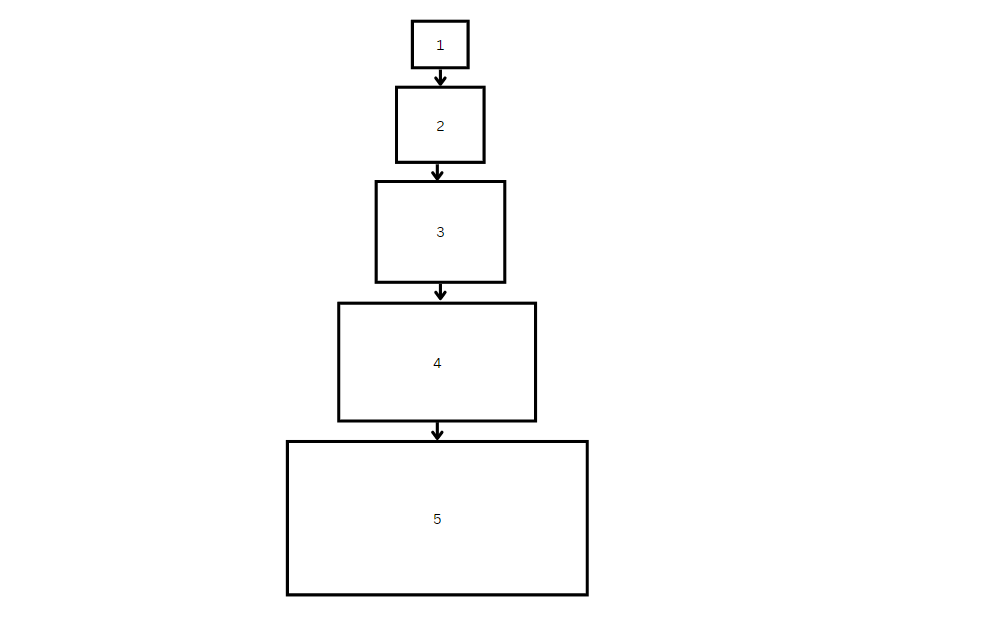
\includegraphics[scale=0.5, trim={0 .8cm 4cm 0cm},clip]{thesistemplate_2020-04-24/chapters/ch1 diagrams/cachesunFinal.png}
    \caption{A cache structure}
    \label{fig:my_label}
\end{figure}

In Figure 1.1, there are five levels of memory that grow physically larger as their level increases. This increase in size allows these higher levels to store more data but at the cost of the speed that the lower levels have. These levels are called caches. The problem with this approach is that caching only improves performance if the data being requested is in small fast memory. This is because, if the data is not in the small memory we must return to the state of a large slow memory.  


Since these small and fast caches can only store a subset of the data in the main memory, how do we ensure they store the requested data? They do this by taking advantage of a property called locality. Locality states that programs are likely to do two things: they are likely to reaccess data they have recently accessed and they are likely to access data near where they are accessing. This property means that the amount of data being accessed is usually small. 

Although we know that there is likely a small amount of relevant data, we still need to determine which data is relevant. In addition to this relevant data, caches quickly fill up with data that is not going to be relevant to future computations. When caches become full, decisions must be made regarding what data to keep versus what to discard from the cache. This process is called eviction.

These eviction decisions are done using cache algorithms, these algorithms decide what data is kept in the cache. There are many types of caches, which has led to a wide variety of cache algorithms with many different focuses.


When designing caching systems we would like to consider a variety of different design choices including which algorithm to use. However, implementing these choices in order to perform testing is very expensive. To avoid these costs, we turn to theoretical models. 


\section{Caching Models}

%TODO: 
To remove extraneous system details and focus on the problem of replacement, the abstract caching problem was created. It provides a way to analyze algorithms' performance without having to implement them.   

\begin{figure}[h]
    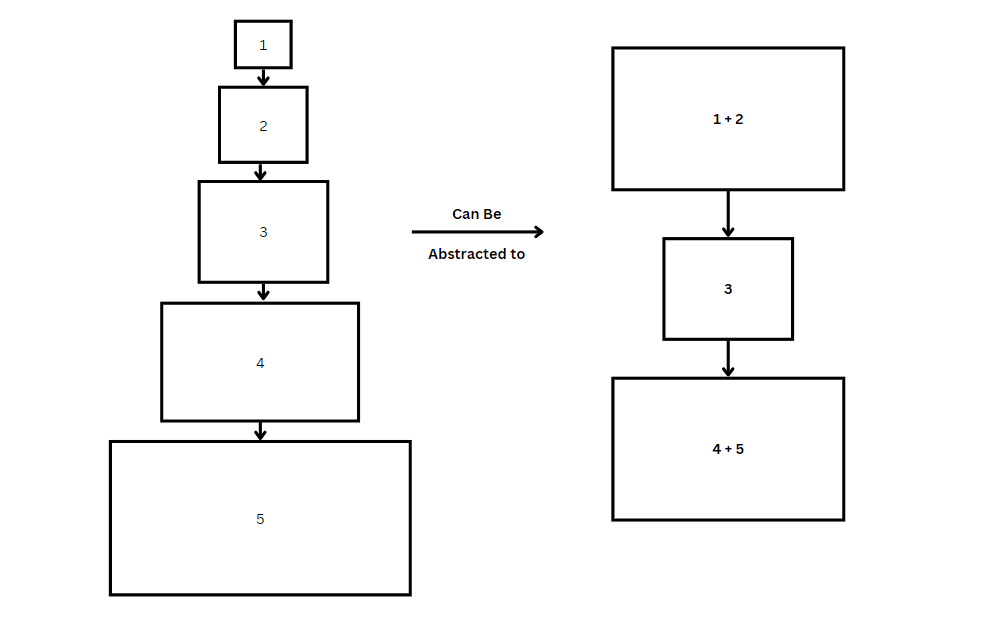
\includegraphics[scale=0.5,  trim={-2cm 0 4cm 0cm},clip]{thesistemplate_2020-04-24/chapters/ch1 diagrams/cachesabFinal.png}
    \caption{How we can view an abstract cache}
    \label{fig:my_label}
\end{figure}



Figure 1.1 shows a system with five levels of caches. An inefficient way to analyze this system would be to look at all five levels and their associated performances. Thinking of caches in the abstract frees us from having to look at all five levels of the cache. Instead, we choose one level of the cache and look at how it performs on a given trace of requests.


In Figure 1.2, we look at level 3 in the abstract model. Since we are focusing just on level 3, we only care about the requests that level 3 handles. This means we can abstract levels 1 and 2 into a single level, as they either already contained the requested data, or it wasn't present. If they contained the data, level 3 never sees the request regardless of which level contained it. Whereas if they didn't level 3 gets this request. We can use this same logic to abstract levels 4 and 5. Because we only care about level 3 and its performance, if level 3 didn't contain the data requested it doesn't matter if it is contained in level 4 or 5.

The abstract caching problem focuses on a cache of size $k$ given a trace $\sigma = \{i_{0}...i_{n} \}$, where each $i$ is requested one at a time in the order of the trace. Every item $i$ has an associated size $S(i)$ and cost $C(i)$. When an item is requested in this problem, the system can't proceed until the item is in the cache. While loading items, the total size of items in the cache can never exceed $k$
When items are requested, if the item is not in the cache, it must pay cost $C(i)$. For an item to fit in a cache, it must first evict items until it has $S(i)$ room.


 
\subsection{The Paging Model}
In the paging model, $\forall i \in \sigma  \text{ }cost(i) =  size(i)=1$. This means that on any given trace, all items' costs and sizes are equal. This model was introduced by \cite{sleator1985amortized} and was created to study cache storage. It allows researchers to look at processor caches wherein there is no size variation because the data is stored in the same size blocks. The cost of retrieving elements from memory is not considered as important as missing a request. 

\subsection{The Cost Model}
In the cost model, $\forall i \in \sigma \text{ } cost(i) =n \text{, } size(i)=1$. This means that any given trace, items will all have the same size, but can vary in cost. This was created by \cite{young1994k} to study the online k server problem in a new model. This model is useful for processor caches, where the size of items is always the same. Unlike the paging model, it can take into account the actual cost it takes to search for items in shared memory.


\subsection{The Fault Model}
In the fault model, $\forall i \in \sigma \text{ } cost(i) = 1\text{, } size(i)=(0\text{ to }k)$. This means that items will have a set cost, but can vary in size. This model was introduced by \cite{irani1997page} and was made to focus on the study of algorithms in web systems. This allows researchers to look at web caches, as the cost of a miss is so large on any item that they can all be considered equal.

\subsection{The Bit Model}
In the bit model, when given $\sigma$, $\forall i \text{ }cost(i)=size(i)$. This model was first introduced by \cite{irani1997page}. This means that items will have a cost that is equal to size. Irani created the model to study the effects of caching algorithms on web caches, but unlike the fault model, the cost difference can be taken into account. This allows bandwidth to be taken into consideration as larger files cost more to transfer.


\subsection{General Model}
In the general model of caching, when given $\sigma$, $\forall i, \textbf{ }  Cost(i) \text{, } Size(i)$. The sizes and costs are not constant between these different items, meaning that on any given trace, the items' sizes and costs can vary. This flexibility comes with an increase in complexity as in this model algorithms must balance the cost of items versus their size.
%Layout should be in the intro 

%Make it more organze, cohesive structure, 
%I am jumping from one thing to another, not sentences making sense. REad it carefully. Bridge the gap 
%make the discussion of layers as abstract as posible
%here are some things that could be 
%talk abstract because my solution is abstract. 
%curretly making processor caches sound like the improtant part. It isnt important! you fuck

%Make this its chapter 

\chapter{Processor Caches}

In this paper, we will be explaining caches through the lens of a processor cache. Most processor caches have three main levels, the L1 cache, being the smallest, the L2 cache, and the L3 cache.


When the processor requests data, it first checks the L1 cache. If the data is in the cache, it is retrieved from there, and the processor can continue processing. If not, the computer checks the L2 cache. If it is not retrieved, it repeats the process again for the L3 cache and either retrieves the data, or it must go to its original location in the memory. Each of these levels has an ever-increasing cost of retrieval, so making sure the items are in the L1 cache as often as possible is important to keep systems running efficiently. 


From Chapter 1 we know that looking at the entire system is not always helpful, so instead we will be looking at the individual level of the cache system.
A processor cache is organized into sets where data blocks can be stored.
Each of these sets can contain singular or multiple cache lines. Each cache line can store a data block and has associated metadata. In the cache line, there is an offset pointing to a location in the data block. This metadata is a tag that is used as an identifier for data and additional metadata that is used by the cache controller to manage the cache line.

\begin{figure}[h]
    \centering
    \caption{An example Cache Line}
    \label{fig:my_label}
    \begin{tikzpicture}
        \node[draw, minimum width=3mm, minimum height=3mm](block) {
        \begin{tikzpicture}
            \node[draw, minimum width=8mm, minimum height=6mm,above= 0mm, right =-\pgflinewidth, label=above:valid] (valid) {0};
            \node[draw, minimum width=20mm, minimum height=5mm, right=-\pgflinewidth of valid,, label=above:tag] (tag) {empty};
            \node[draw, minimum width=40mm, minimum height=5mm, right=-\pgflinewidth of tag, label=above:data] (data) {empty};
        \end{tikzpicture}
        };
    \end{tikzpicture}
\end{figure}


When a cache receives a request, which is a memory location, it must decode what that request is for. To do this, it breaks the request into the offset, set, and tag. The offset starts at the least significant bit and points to a specific location in the data block. Next, the cache uses the set bits to determine which set this data block can be put in. The remaining bits are the tag, which is used as an identifier. Each cache line also has an associated valid bit to identify the data block's validity.

After breaking these requests into their parts, the cache must insert the data block into the correct location if it is not already there. To do this, it strips the set bits from the request and uses it to locate the set within the cache in which the data block can be put. Then, it checks the tag of each line in the set to see if the data block is already in one of the set's cache lines because blocks can be in the same cache line. If the data is not in the cache, then the cache must evict if full.



\section{Associativity of Caches}
Associativity in caches affects the number of elements per set in the cache. Caches with high associativity have fewer sets while caches with low associativity have more sets. The three kinds of cache associativity in caches are fully associative, set-associative, and direct-mapped. What kind of associativity a cache has is important to system performance. This is through two main factors: One, every additional cache line in a set causes an increased time to search when an item is requested. And two, when there are too few lines in a set, evictions occur more often which causes a time penalty as items must continually be retrieved from memory.



\subsection{Fully-Associative Cache}

A fully associative cache is a type of cache organization where the entire cache is one set, meaning that any data block can be stored in any cache line. This approach allows for maximum flexibility in cache organization because any available cache line can store an incoming data block, making efficient use of cache space.

\begin{figure}[H]
    \centering
    \caption{Structure of a fully associative cache}
    \label{fig:my_label}
\begin{tikzpicture}
\node[draw, minimum width=15mm, minimum height=10mm](block) {
\begin{tikzpicture}
\node[draw, minimum width=8mm, minimum height=6mm,above= 0mm, right =-\pgflinewidth, label=above:valid] (valid) {0};
\node[draw, minimum width=20mm, minimum height=5mm, right=-\pgflinewidth of valid,, label=above:tag] (tag) {empty};
\node[draw, minimum width=40mm, minimum height=5mm, right=-\pgflinewidth of tag, label=above:data] (data) {empty};
\node[draw, minimum width=8mm, minimum height=6mm,below= 0mm of valid] (valid) {0};
\node[draw, minimum width=20mm, minimum height=5mm, right=-\pgflinewidth of valid] (tag) {empty};
\node[draw, minimum width=40mm, minimum height=5mm, right=-\pgflinewidth of tag] (data) {empty};
\node[draw, minimum width=8mm, minimum height=6mm,below= 0mm of valid] (valid) {0};
\node[draw, minimum width=20mm, minimum height=5mm, right=-\pgflinewidth of valid] (tag) {empty};
\node[draw, minimum width=40mm, minimum height=5mm, right=-\pgflinewidth of tag] (data) {empty};
\node[draw, minimum width=8mm, minimum height=6mm,below= 0mm of valid] (valid) {0};
\node[draw, minimum width=20mm, minimum height=5mm, right=-\pgflinewidth of valid] (tag) {empty};
\node[draw, minimum width=40mm, minimum height=5mm, right=-\pgflinewidth of tag] (data) {empty};
\node[draw, minimum width=8mm, minimum height=6mm,below= 0mm of valid] (valid) {0};
\node[draw, minimum width=20mm, minimum height=5mm, right=-\pgflinewidth of valid] (tag) {empty};
\node[draw, minimum width=40mm, minimum height=5mm, right=-\pgflinewidth of tag] (data) {empty};
\node[draw, minimum width=8mm, minimum height=6mm,below= 0mm of valid] (valid) {0};
\node[draw, minimum width=20mm, minimum height=5mm, right=-\pgflinewidth of valid] (tag) {empty};
\node[draw, minimum width=40mm, minimum height=5mm, right=-\pgflinewidth of tag] (data) {empty};
\node[draw, minimum width=8mm, minimum height=6mm,below= 0mm of valid] (valid) {0};
\node[draw, minimum width=20mm, minimum height=5mm, right=-\pgflinewidth of valid] (tag) {empty};
\node[draw, minimum width=40mm, minimum height=5mm, right=-\pgflinewidth of tag] (data) {empty};
\node[draw, minimum width=8mm, minimum height=6mm,below= 0mm of valid] (valid) {0};
\node[draw, minimum width=20mm, minimum height=5mm, right=-\pgflinewidth of valid] (tag) {empty};
\node[draw, minimum width=40mm, minimum height=5mm, right=-\pgflinewidth of tag] (data) {empty};

\end{tikzpicture}
};


\node[draw, minimum width=15mm, right = 0cm of block, minimum height=10mm,label=above:0x0010](reqs) {
    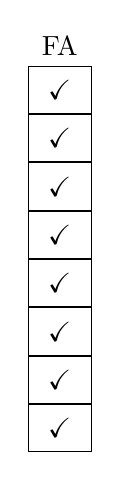
\begin{tikzpicture}
        \node[draw, minimum width=8mm, minimum height=6mm, label=above:FA] (set) {\checkmark};
        \node[draw, minimum width=8mm, minimum height=6mm, below = 0mm of set] (set) {\checkmark};
        \node[draw, minimum width=8mm, minimum height=6mm, below = 0mm of set] (set) {\checkmark};
        \node[draw, minimum width=8mm, minimum height=6mm, below = 0mm of set] (set) {\checkmark};
        \node[draw, minimum width=8mm, minimum height=6mm, below = 0mm of set] (set) {\checkmark};
        \node[draw, minimum width=8mm, minimum height=6mm, below = 0mm of set] (set) {\checkmark};
        \node[draw, minimum width=8mm, minimum height=6mm, below = 0mm of set] (set) {\checkmark};
        \node[draw, minimum width=8mm, minimum height=6mm, below = 0mm of set] (set) {\checkmark};
    \end{tikzpicture}
};






\end{tikzpicture}
\end{figure}
This organization comes with the cost that every cache line must be searched when trying to find the data block in the cache. This increased number of searches results in longer access times than other cache memory organizations.

\subsection{Direct-Mapped Cache}

In a direct-mapped cache, every cache line is its own set. When a cache receives a request, it can quickly check the corresponding cache line to see if the data block is already present. This approach allows for fast cache look-ups because there is only one possible location where a given data block can be stored in the cache.
\begin{figure}[h]
\caption{A structure of a direct mapped cache}
\centering
\begin{tikzpicture}
\node[draw, minimum width=15mm, minimum height=10mm](block) {
\begin{tikzpicture}

\node[draw, minimum width=8mm, minimum height=6mm, label=above:set] (set) {0};
\node[draw, minimum width=8mm, minimum height=6mm,right= .8cm of set, label=above:valid] (valid) {0};
\node[draw, minimum width=20mm, minimum height=5mm, right=-\pgflinewidth of valid, label=above:tag] (tag) {empty};
\node[draw, minimum width=40mm, minimum height=5mm, right=-\pgflinewidth of tag, label=above:data] (data) {empty};
\node[draw, minimum width=8mm, minimum height=6mm, below= 0mm of set] (set) {1};
\node[draw, minimum width=8mm, minimum height=6mm, right =.8cm of set] (valid) {0};
\node[draw, minimum width=20mm, minimum height=5mm,below= 0mm of set, right=-\pgflinewidth of valid] (tag) {empty};
\node[draw, minimum width=40mm, minimum height=5mm,below= 0mm of set, right=-\pgflinewidth of tag] (data) {empty};
\node[draw, minimum width=8mm, minimum height=6mm, below= 0mm of set] (set) {2};
\node[draw, minimum width=8mm, minimum height=6mm, right =.8cm of set] (valid) {0};
\node[draw, minimum width=20mm, minimum height=5mm,below= 0mm of set, right=-\pgflinewidth of valid] (tag) {empty};
\node[draw, minimum width=40mm, minimum height=5mm,below= 0mm of set, right=-\pgflinewidth of tag] (data) {empty};\node[draw, minimum width=8mm, minimum height=6mm, below= 0mm of set] (set) {3};
\node[draw, minimum width=8mm, minimum height=6mm, right =.8cm of set] (valid) {0};
\node[draw, minimum width=20mm, minimum height=5mm,below= 0mm of set, right=-\pgflinewidth of valid] (tag) {empty};
\node[draw, minimum width=40mm, minimum height=5mm,below= 0mm of set, right=-\pgflinewidth of tag] (data) {empty};
\node[draw, minimum width=8mm, minimum height=6mm, below= 0mm of set] (set) {4};
\node[draw, minimum width=8mm, minimum height=6mm, right =.8cm of set] (valid) {0};
\node[draw, minimum width=20mm, minimum height=5mm,below= 0mm of set, right=-\pgflinewidth of valid] (tag) {empty};
\node[draw, minimum width=40mm, minimum height=5mm,below= 0mm of set, right=-\pgflinewidth of tag] (data) {empty};
\node[draw, minimum width=8mm, minimum height=6mm, below= 0mm of set] (set) {5};
\node[draw, minimum width=8mm, minimum height=6mm, right =.8cm of set] (valid) {0};
\node[draw, minimum width=20mm, minimum height=5mm,below= 0mm of set, right=-\pgflinewidth of valid] (tag) {empty};
\node[draw, minimum width=40mm, minimum height=5mm,below= 0mm of set, right=-\pgflinewidth of tag] (data) {empty};
\node[draw, minimum width=8mm, minimum height=6mm, below= 0mm of set] (set) {6};
\node[draw, minimum width=8mm, minimum height=6mm, right =.8cm of set] (valid) {0};
\node[draw, minimum width=20mm, minimum height=5mm,below= 0mm of set, right=-\pgflinewidth of valid] (tag) {empty};
\node[draw, minimum width=40mm, minimum height=5mm,below= 0mm of set, right=-\pgflinewidth of tag] (data) {empty};
\node[draw, minimum width=8mm, minimum height=6mm, below= 0mm of set] (set) {7};
\node[draw, minimum width=8mm, minimum height=6mm, right =.8cm of set] (valid) {0};
\node[draw, minimum width=20mm, minimum height=5mm,below= 0mm of set, right=-\pgflinewidth of valid] (tag) {empty};
\node[draw, minimum width=40mm, minimum height=5mm,below= 0mm of set, right=-\pgflinewidth of tag] (data) {empty};
\end{tikzpicture}
};

\node[draw, minimum width=15mm, right = 0cm of block, minimum height=10mm,label=above:0x5371](reqs) {
    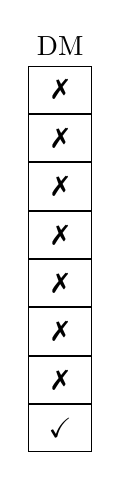
\begin{tikzpicture}
        \node[draw, minimum width=8mm, minimum height=6mm, label=above:DM] (set) {\xmark};
        \node[draw, minimum width=8mm, minimum height=6mm, below = 0mm of set] (set) {\xmark};
        \node[draw, minimum width=8mm, minimum height=6mm, below = 0mm of set] (set) {\xmark};
        \node[draw, minimum width=8mm, minimum height=6mm, below = 0mm of set] (set) {\xmark};
        \node[draw, minimum width=8mm, minimum height=6mm, below = 0mm of set] (set) {\xmark};
        \node[draw, minimum width=8mm, minimum height=6mm, below = 0mm of set] (set) {\xmark};
        \node[draw, minimum width=8mm, minimum height=6mm, below = 0mm of set] (set) {\xmark};
        \node[draw, minimum width=8mm, minimum height=6mm, below = 0mm of set] (set) {\checkmark};
    \end{tikzpicture}
};


\end{tikzpicture}
\end{figure}


This simplicity makes direct-mapped caches efficient, but they can suffer from a problem known as thrashing. This is where different data blocks map to the same cache line repeatedly, causing frequent cache misses and degrading performance. 

\subsection{Set-Associative Cache}

An x-way set associative cache is a type of cache memory organization that falls between the direct-mapped and fully associative approaches. In set-associative caching, a cache line is part of a set, with each set containing multiple cache lines. When a request is made, its associated data block is stored in one of the cache lines within the corresponding set. The set bits determine which set the request maps to and then search for an empty line within that set. If no empty lines are available, the cache controller selects one of the existing lines within the set to replace.


\begin{figure}[H]
    \centering
    \caption{Structure of a 2-way set associative cache}
    \label{fig:my_label}
\begin{tikzpicture}
\node[draw, minimum width=15mm, minimum height=10mm](block) {
\begin{tikzpicture}
\node[draw, minimum width=8mm, minimum height=6mm, label=above:set] (set) {0};
\node[draw, minimum width=8mm, minimum height=6mm,above= 0mm of set, right =.8cm of set,, label=above:valid] (valid) {0};
\node[draw, minimum width=20mm, minimum height=5mm, right=-\pgflinewidth of valid,, label=above:tag] (tag) {empty};
\node[draw, minimum width=40mm, minimum height=5mm, right=-\pgflinewidth of tag, label=above:data] (data) {empty};
\node[draw, minimum width=8mm, minimum height=6mm, below= 0mm of set] (set) {0};
\node[draw, minimum width=8mm, minimum height=6mm, right =.8cm of set] (valid) {0};
\node[draw, minimum width=20mm, minimum height=5mm,below= 0mm of set, right=-\pgflinewidth of valid] (tag) {empty};
\node[draw, minimum width=40mm, minimum height=5mm,below= 0mm of set, right=-\pgflinewidth of tag] (data) {empty};
\node[draw, minimum width=8mm, minimum height=6mm, below= 0mm of set] (set) {1};
\node[draw, minimum width=8mm, minimum height=6mm, right = 0.8cm of set] (valid) {0};
\node[draw, minimum width=20mm, minimum height=5mm,below= 0mm of set, right=-\pgflinewidth of valid] (tag) {empty};
\node[draw, minimum width=40mm, minimum height=5mm,below= 0mm of set, right=-\pgflinewidth of tag] (data) {empty};\node[draw, minimum width=8mm, minimum height=6mm, below= 0mm of set] (set) {1};
\node[draw, minimum width=8mm, minimum height=6mm, right =.8cm of set] (valid) {0};
\node[draw, minimum width=20mm, minimum height=5mm,below= 0mm of set, right=-\pgflinewidth of valid] (tag) {empty};
\node[draw, minimum width=40mm, minimum height=5mm,below= 0mm of set, right=-\pgflinewidth of tag] (data) {empty};\node[draw, minimum width=8mm, minimum height=6mm, below= 0mm of set] (set) {2};
\node[draw, minimum width=8mm, minimum height=6mm, right =0.8cm of set] (valid) {0};
\node[draw, minimum width=20mm, minimum height=5mm,below= 0mm of set, right=-\pgflinewidth of valid] (tag) {empty};
\node[draw, minimum width=40mm, minimum height=5mm,below= 0mm of set, right=-\pgflinewidth of tag] (data) {empty};
\node[draw, minimum width=40mm, minimum height=5mm,below= 0mm of set, right=-\pgflinewidth of tag] (data) {empty};\node[draw, minimum width=8mm, minimum height=6mm, below= 0mm of set] (set) {2};
\node[draw, minimum width=8mm, minimum height=6mm, right =0.8cm of set] (valid) {0};
\node[draw, minimum width=20mm, minimum height=5mm,below= 0mm of set, right=-\pgflinewidth of valid] (tag) {empty};
\node[draw, minimum width=40mm, minimum height=5mm,below= 0mm of set, right=-\pgflinewidth of tag] (data) {empty};
\node[draw, minimum width=8mm, minimum height=6mm, below= 0mm of set] (set) {3};
\node[draw, minimum width=8mm, minimum height=6mm, right =.8cm of set] (valid) {0};
\node[draw, minimum width=20mm, minimum height=5mm,below= 0mm of set, right=-\pgflinewidth of valid] (tag) {empty};
\node[draw, minimum width=40mm, minimum height=5mm,below= 0mm of set, right=-\pgflinewidth of tag] (data) {empty};
\node[draw, minimum width=8mm, minimum height=6mm, below= 0mm of set] (set) {3};
\node[draw, minimum width=8mm, minimum height=6mm, right =.8cm of set] (valid) {0};
\node[draw, minimum width=20mm, minimum height=5mm,below= 0mm of set, right=-\pgflinewidth of valid] (tag) {empty};
\node[draw, minimum width=40mm, minimum height=5mm,below= 0mm of set, right=-\pgflinewidth of tag] (data) {empty};
\end{tikzpicture}
};

\node[draw, minimum width=15mm, right = 0cm of block, minimum height=10mm,label=above:0xDB1F](reqs) {
    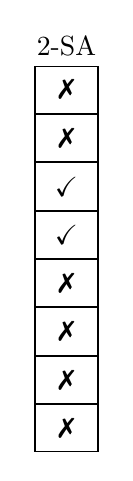
\begin{tikzpicture}
        \node[draw, minimum width=8mm, minimum height=6mm, label=above:2-SA] (set) {\xmark};
        \node[draw, minimum width=8mm, minimum height=6mm, below = 0mm of set] (set) {\xmark};
        \node[draw, minimum width=8mm, minimum height=6mm, below = 0mm of set] (set) {\checkmark};
        \node[draw, minimum width=8mm, minimum height=6mm, below = 0mm of set] (set) {\checkmark};
        \node[draw, minimum width=8mm, minimum height=6mm, below = 0mm of set] (set) {\xmark};
        \node[draw, minimum width=8mm, minimum height=6mm, below = 0mm of set] (set) {\xmark};
        \node[draw, minimum width=8mm, minimum height=6mm, below = 0mm of set] (set) {\xmark};
        \node[draw, minimum width=8mm, minimum height=6mm, below = 0mm of set] (set) {\xmark};
    \end{tikzpicture}
};

\end{tikzpicture}
\end{figure}
Set-associative caching offers a middle ground between fully associative and direct mapped caching, where a 1-way set is a direct mapped cache and k-way is a fully associative cache. This gives it flexibility as the entire cache doesn't need to be searched for every request, but it can still struggle with thrashing.

\section{Decoding Explanation}
Figure 2.5 shows how a processor deals with a request to an address called 0xABCD. This example shows how the address is decomposed, the cache is searched, and eviction is performed to make space to load the data block.

\begin{figure}[h]
    \centering
    \caption{How a fully associative cache decodes a request}
    \label{fig:my_label}
\begin{tikzpicture}
\node[text width = 10cm, above = 0cm of block](texter) {The cache has a block size of 16 bytes and the cache can store 128 bytes of data caching this sequence: \\ \textbf{0xABCD} };
    \node[draw, minimum width = 5 cm, below = 1cm of texter](frt){1010101111001101};
    \node[draw, minimum width = 5 cm,text width =5 cm, below = 1cm of frt](snd){Offset bits: $\log_2(16) = 4$\\ Tag bits:$16 - 4 = 12$};
    \node[draw, below = 1cm of snd](trd){
    1010 1011 1100 1101 
    };
    \node[label = below:Offset, below right= 0cm of trd, minimum width = 1 cm, minimum height= .7 cm, draw] at (.9,-1.6){};
    \node[label = below:Tag, below left = 0cm of trd.south, minimum width = 3 cm, minimum height= .7 cm, draw] at (.9,-1.6){};
\end{tikzpicture}
\end{figure}


As can be seen in Figure 2.5, when a cache receives a request: First it breaks the requests into their binary representation. Then it uses the $\log_2(\text{block size})$ to find the number of offset bits, ensuring the remaining bits are used for the tag. Once this decoding is complete, the cache stores the data.
\begin{figure}
    \centering
    \caption{Combined figure of how the different associativity of caches can store requests with the cache structure in Figure 2.5}
    \label{fig:my_label}
\begin{tikzpicture}


\node[draw, minimum width=15mm, minimum height=10mm,label=above:0x0010](reqs) {
    \begin{tikzpicture}
        \node[draw, minimum width=8mm, minimum height=6mm, label=above:FA] (set) {\checkmark};
        \node[draw, minimum width=8mm, minimum height=6mm,above= 0mm of set, right =0cm of set, label=above:2SA] (valid) {\xmark};
        \node[draw, minimum width=8mm, minimum height=5mm, right=-\pgflinewidth of valid,, label=above:DM] (tag) {\xmark};
        
        \node[draw, minimum width=8mm, minimum height=6mm, below = 0mm of set] (set) {\checkmark};
        \node[draw, minimum width=8mm, minimum height=6mm,above= 0mm of set, right =0cm of set] (valid) {\xmark};
        \node[draw, minimum width=8mm, minimum height=5mm, right=-\pgflinewidth of valid] (tag) {\xmark};

        \node[draw, minimum width=8mm, minimum height=6mm, below = 0mm of set] (set) {\checkmark};
        \node[draw, minimum width=8mm, minimum height=6mm,above= 0mm of set, right =0cm of set] (valid) {\checkmark};
        \node[draw, minimum width=8mm, minimum height=5mm, right=-\pgflinewidth of valid] (tag) {\checkmark};

        \node[draw, minimum width=8mm, minimum height=6mm, below = 0mm of set] (set) {\checkmark};
        \node[draw, minimum width=8mm, minimum height=6mm,above= 0mm of set, right =0cm of set] (valid) {\checkmark};
        \node[draw, minimum width=8mm, minimum height=5mm, right=-\pgflinewidth of valid] (tag) {\xmark};

        \node[draw, minimum width=8mm, minimum height=6mm, below = 0mm of set] (set) {\checkmark};
        \node[draw, minimum width=8mm, minimum height=6mm,above= 0mm of set, right =0cm of set] (valid) {\xmark};
        \node[draw, minimum width=8mm, minimum height=5mm, right=-\pgflinewidth of valid] (tag) {\xmark};

        \node[draw, minimum width=8mm, minimum height=6mm, below = 0mm of set] (set) {\checkmark};
        \node[draw, minimum width=8mm, minimum height=6mm,above= 0mm of set, right =0cm of set] (valid) {\xmark};
        \node[draw, minimum width=8mm, minimum height=5mm, right=-\pgflinewidth of valid] (tag) {\xmark};
        \node[draw, minimum width=8mm, minimum height=6mm, below = 0mm of set] (set) {\checkmark};
        \node[draw, minimum width=8mm, minimum height=6mm,above= 0mm of set, right =0cm of set] (valid) {\xmark};
        \node[draw, minimum width=8mm, minimum height=5mm, right=-\pgflinewidth of valid] (tag) {\xmark};
        \node[draw, minimum width=8mm, minimum height=6mm, below = 0mm of set] (set) {\checkmark};
        \node[draw, minimum width=8mm, minimum height=6mm,above= 0mm of set, right =0cm of set] (valid) {\xmark};
        \node[draw, minimum width=8mm, minimum height=5mm, right=-\pgflinewidth of valid] (tag) {\xmark};
        
    \end{tikzpicture}
};

\node[minimum width=10mm, minimum height=10mm, below = 1 cm of block](block2) {
};



\node[draw, minimum width=15mm, left = 3cm of reqs, minimum height=10mm,label=above:0x251B](reqs2) {
    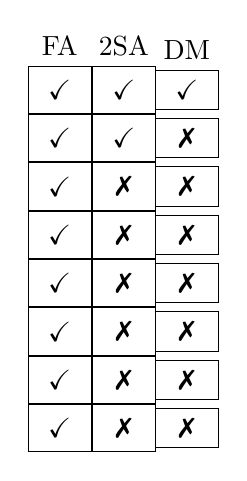
\begin{tikzpicture}
        \node[draw, minimum width=8mm, minimum height=6mm, label=above:FA] (set) {\checkmark};
        \node[draw, minimum width=8mm, minimum height=6mm,above= 0mm of set, right =0cm of set, label=above:2SA] (valid) {\checkmark};
        \node[draw, minimum width=8mm, minimum height=5mm, right=-\pgflinewidth of valid,, label=above:DM] (tag) {\checkmark};
        
        \node[draw, minimum width=8mm, minimum height=6mm, below = 0mm of set] (set) {\checkmark};
        \node[draw, minimum width=8mm, minimum height=6mm,above= 0mm of set, right =0cm of set] (valid) {\checkmark};
        \node[draw, minimum width=8mm, minimum height=5mm, right=-\pgflinewidth of valid] (tag) {\xmark};

        \node[draw, minimum width=8mm, minimum height=6mm, below = 0mm of set] (set) {\checkmark};
        \node[draw, minimum width=8mm, minimum height=6mm,above= 0mm of set, right =0cm of set] (valid) {\xmark};
        \node[draw, minimum width=8mm, minimum height=5mm, right=-\pgflinewidth of valid] (tag) {\xmark};

        \node[draw, minimum width=8mm, minimum height=6mm, below = 0mm of set] (set) {\checkmark};
        \node[draw, minimum width=8mm, minimum height=6mm,above= 0mm of set, right =0cm of set] (valid) {\xmark};
        \node[draw, minimum width=8mm, minimum height=5mm, right=-\pgflinewidth of valid] (tag) {\xmark};
     \node[draw, minimum width=8mm, minimum height=6mm, below = 0mm of set] (set) {\checkmark};
        \node[draw, minimum width=8mm, minimum height=6mm,above= 0mm of set, right =0cm of set] (valid) {\xmark};
        \node[draw, minimum width=8mm, minimum height=5mm, right=-\pgflinewidth of valid] (tag) {\xmark};
     \node[draw, minimum width=8mm, minimum height=6mm, below = 0mm of set] (set) {\checkmark};
        \node[draw, minimum width=8mm, minimum height=6mm,above= 0mm of set, right =0cm of set] (valid) {\xmark};
        \node[draw, minimum width=8mm, minimum height=5mm, right=-\pgflinewidth of valid] (tag) {\xmark};
\node[draw, minimum width=8mm, minimum height=6mm, below = 0mm of set] (set) {\checkmark};
        \node[draw, minimum width=8mm, minimum height=6mm,above= 0mm of set, right =0cm of set] (valid) {\xmark};
        \node[draw, minimum width=8mm, minimum height=5mm, right=-\pgflinewidth of valid] (tag) {\xmark};
\node[draw, minimum width=8mm, minimum height=6mm, below = 0mm of set] (set) {\checkmark};
        \node[draw, minimum width=8mm, minimum height=6mm,above= 0mm of set, right =0cm of set] (valid) {\xmark};
        \node[draw, minimum width=8mm, minimum height=5mm, right=-\pgflinewidth of valid] (tag) {\xmark};

        
    \end{tikzpicture}
};


\node[minimum width=10mm, minimum height=10mm, left = 3cm of block2](block3) {
};

\node[draw, minimum width=15mm, left = 3cm of reqs2, minimum height=10mm,label=above:0xFF0F](reqs3) {
    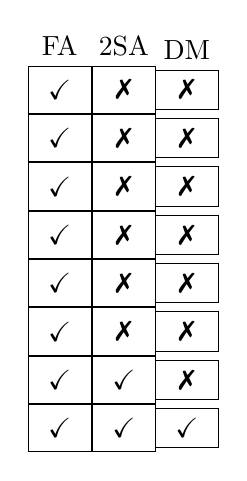
\begin{tikzpicture}        \node[draw, minimum width=8mm, minimum height=6mm, label=above:FA] (set) {\checkmark};
        \node[draw, minimum width=8mm, minimum height=6mm,above= 0mm of set, right =0cm of set, label=above:2SA] (valid) {\xmark};
        \node[draw, minimum width=8mm, minimum height=5mm, right=-\pgflinewidth of valid,, label=above:DM] (tag) {\xmark};
        
        \node[draw, minimum width=8mm, minimum height=6mm, below = 0mm of set] (set) {\checkmark};
        \node[draw, minimum width=8mm, minimum height=6mm,above= 0mm of set, right =0cm of set] (valid) {\xmark};
        \node[draw, minimum width=8mm, minimum height=5mm, right=-\pgflinewidth of valid] (tag) {\xmark};

        \node[draw, minimum width=8mm, minimum height=6mm, below = 0mm of set] (set) {\checkmark};
        \node[draw, minimum width=8mm, minimum height=6mm,above= 0mm of set, right =0cm of set] (valid) {\xmark};
        \node[draw, minimum width=8mm, minimum height=5mm, right=-\pgflinewidth of valid] (tag) {\xmark};

        \node[draw, minimum width=8mm, minimum height=6mm, below = 0mm of set] (set) {\checkmark};
        \node[draw, minimum width=8mm, minimum height=6mm,above= 0mm of set, right =0cm of set] (valid) {\xmark};
        \node[draw, minimum width=8mm, minimum height=5mm, right=-\pgflinewidth of valid] (tag) {\xmark};

        \node[draw, minimum width=8mm, minimum height=6mm, below = 0mm of set] (set) {\checkmark};
        \node[draw, minimum width=8mm, minimum height=6mm,above= 0mm of set, right =0cm of set] (valid) {\xmark};
        \node[draw, minimum width=8mm, minimum height=5mm, right=-\pgflinewidth of valid] (tag) {\xmark};

        \node[draw, minimum width=8mm, minimum height=6mm, below = 0mm of set] (set) {\checkmark};
        \node[draw, minimum width=8mm, minimum height=6mm,above= 0mm of set, right =0cm of set] (valid) {\xmark};
        \node[draw, minimum width=8mm, minimum height=5mm, right=-\pgflinewidth of valid] (tag) {\xmark};

        \node[draw, minimum width=8mm, minimum height=6mm, below = 0mm of set] (set) {\checkmark};
        \node[draw, minimum width=8mm, minimum height=6mm,above= 0mm of set, right =0cm of set] (valid) {\checkmark};
        \node[draw, minimum width=8mm, minimum height=5mm, right=-\pgflinewidth of valid] (tag) {\xmark};

        \node[draw, minimum width=8mm, minimum height=6mm, below = 0mm of set] (set) {\checkmark};
        \node[draw, minimum width=8mm, minimum height=6mm,above= 0mm of set, right =0cm of set] (valid) {\checkmark};
        \node[draw, minimum width=8mm, minimum height=5mm, right=-\pgflinewidth of valid] (tag) {\checkmark};
        
    \end{tikzpicture}
};
\end{tikzpicture}
\end{figure}

\chapter{Caching Algorithms}
Caching algorithms are used to manage the content of a cache when dealing with a series of requests from a computer. When the cache becomes full, these algorithms decide which pieces of data to evict. The eviction policy is different for every algorithm, but the general goal is the same, to minimize the cost of cache misses as they decrease the overall performance of the system.


\section{Least Recently Used}


The Least Recently Used(LRU) algorithm has an intuitive structure and a relatively simple implementation. When choosing which item to evict from a cache, it evicts the item least recently referenced. This means that when LRU decides to evict something from the cache, it looks at the trace from the current request back to the start of the trace and chooses the item which is currently in the cache whose most recent reference is farthest from the current request. This makes LRU well-suited for applications where a small set of items are accessed together as it keeps items frequently accessed in the cache.


Figure 3.1 is a basic example of how LRU works given a simple trace. LRU functions exceptionally well on this trace, only missing on the first occurrence of an item due to the trace's tendency to request a subset of items frequently. This means that due to the lack of misses on this trace given LRU, this cache would cause a minimal performance penalty as it only misses items it hasn't seen yet. 
\begin{figure}[H]
    \centering
    \caption{LRU cache given: A,B,C,D,B,C,D}
    \label{fig:my_label}
\begin{tikzpicture}
\node[rounded corners,draw=black,label=above:LRU, minimum size=2cm] (a) at (0,0)  {
    \begin{tikzpicture}
        \node[rounded corners,draw=black,minimum size=0.8cm]{A};
    \end{tikzpicture}
    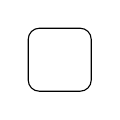
\begin{tikzpicture}
        \node[rounded corners,draw=black,minimum size=0.8cm]{};
    \end{tikzpicture}
    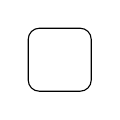
\begin{tikzpicture}
        \node[rounded corners,draw=black,minimum size=0.8cm]{};
    \end{tikzpicture}
    };
    \node[text width=3cm] at (-3, 0) 
    {Miss on A as first instance, add A to cache};

    
    \node[rounded corners,draw=black,minimum size=2cm] (b) at (0,-2.5)  {   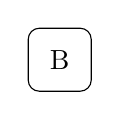
\begin{tikzpicture}
        \node[rounded corners,draw=black,minimum size=0.8cm]{B};
    \end{tikzpicture}
    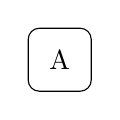
\begin{tikzpicture}
        \node[rounded corners,draw=black,minimum size=0.8cm]{A};
    \end{tikzpicture}
    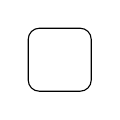
\begin{tikzpicture}
        \node[rounded corners,draw=black,minimum size=0.8cm]{};
    \end{tikzpicture}
    };
     \node[text width=3cm] at (-3,-2.5) 
    {Miss on B as first instance, add B to cache};
    
    \node[rounded corners,draw=black,minimum size=2cm] (c) at (0,-5)  {   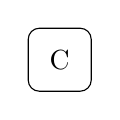
\begin{tikzpicture}
        \node[rounded corners,draw=black,minimum size=0.8cm]{C};
    \end{tikzpicture}
    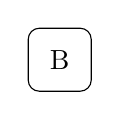
\begin{tikzpicture}
        \node[rounded corners,draw=black,minimum size=0.8cm]{B};
    \end{tikzpicture}
    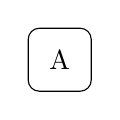
\begin{tikzpicture}
        \node[rounded corners,draw=black,minimum size=0.8cm]{A};
    \end{tikzpicture}
    };

    \node[text width=3cm] at (-3,-5) 
    {Miss on C as first instance, C added to cache};
      
    \node[rounded corners,draw=black,minimum size=2cm] (d) at (0,-7.5)  {   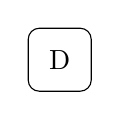
\begin{tikzpicture}
        \node[rounded corners,draw=black,minimum size=0.8cm]{D};
    \end{tikzpicture}
    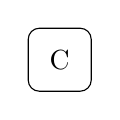
\begin{tikzpicture}
        \node[rounded corners,draw=black,minimum size=0.8cm]{C};
    \end{tikzpicture}
    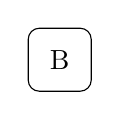
\begin{tikzpicture}
        \node[rounded corners,draw=black,minimum size=0.8cm]{B};
    \end{tikzpicture}
    };

     \node[text width=3cm] at (-3,-7.5) 
    {Miss on D as first instance, evict A since LRU};
    
    \node[rounded corners,draw=black,minimum size=2cm, below left=1 cm of d] (e) at (2.2,-8.4)  { 
    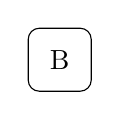
\begin{tikzpicture}
        \node[rounded corners,draw=black,minimum size=0.8cm]{B};
    \end{tikzpicture}
    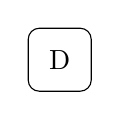
\begin{tikzpicture}
        \node[rounded corners,draw=black,minimum size=0.8cm]{D};
    \end{tikzpicture}
    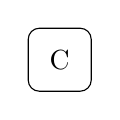
\begin{tikzpicture}
        \node[rounded corners,draw=black,minimum size=0.8cm]{C};
    \end{tikzpicture}
    };  

     \node[text width=3cm] at (-3,-10) 
    {Hit on B};

    \node[rounded corners,draw=black,minimum size=2cm, below left=1 cm of d] (f) at (2.2,-11)  { 
    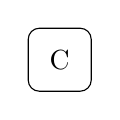
\begin{tikzpicture}
        \node[rounded corners,draw=black,minimum size=0.8cm]{C};
    \end{tikzpicture}
    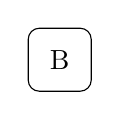
\begin{tikzpicture}
        \node[rounded corners,draw=black,minimum size=0.8cm]{B};
    \end{tikzpicture}
    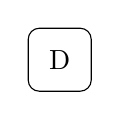
\begin{tikzpicture}
        \node[rounded corners,draw=black,minimum size=0.8cm]{D};
    \end{tikzpicture}
    };  

     \node[text width=3cm] at (-3,-12.5) 
    {Hit on C};

    \node[rounded corners,draw=black,minimum size=2cm, below left=1 cm of d] (g) at (2.2,-13.5)  { 
    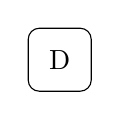
\begin{tikzpicture}
        \node[rounded corners,draw=black,minimum size=0.8cm]{D};
    \end{tikzpicture}
    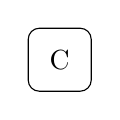
\begin{tikzpicture}
        \node[rounded corners,draw=black,minimum size=0.8cm]{C};
    \end{tikzpicture}
    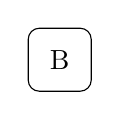
\begin{tikzpicture}
        \node[rounded corners,draw=black,minimum size=0.8cm]{B};
    \end{tikzpicture}
    };  

     \node[text width=3cm] at (-3,-15) 
    {Hit on D};

    \draw[thick,->] (a) -- (b);
    \draw[thick,->](b) -- (c);  
    \draw[thick,->](c) -- (d);  
    \draw[thick,->](d) -- (e);  
    \draw[thick,->](e) -- (f);  
    \draw[thick,->](f) -- (g);  
\end{tikzpicture}
\end{figure}



\section{Most Recently Used}
The Most Recently Used (MRU) algorithm is an algorithm that when a cache becomes full of items, evicts the most recently used item. This means that when needing to evict an item, MRU evicts the last item that was requested just before the current request. This makes MRU suited for traces where items referenced furthest in the past are more likely to be requested again than those accessed more recently.

Figure 3.2 is a basic example of how MRU works. On this trace, MRU only misses the first instance of an item as, after the first instance of an item, the cache is unlikely to see it accessed again soon, as A in this trace. 

\begin{figure}[H]
    \centering
    \caption{MRU cache given: A,B,C,D,B,D,A}
    \label{fig:my_label}
\begin{tikzpicture}
\node[rounded corners,draw=black,label=above:MRU, minimum size=2cm] (a) at (0,0)  {
    \begin{tikzpicture}
        \node[rounded corners,draw=black,minimum size=0.8cm]{A};
    \end{tikzpicture}
    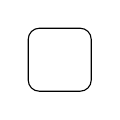
\begin{tikzpicture}
        \node[rounded corners,draw=black,minimum size=0.8cm]{};
    \end{tikzpicture}
    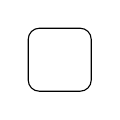
\begin{tikzpicture}
        \node[rounded corners,draw=black,minimum size=0.8cm]{};
    \end{tikzpicture}
    };
    \node[text width=3cm] at (-3, 0) 
    {Miss on A as first instance, add A to cache};

    
    \node[rounded corners,draw=black,minimum size=2cm] (b) at (0,-2.5)  {   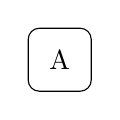
\begin{tikzpicture}
        \node[rounded corners,draw=black,minimum size=0.8cm]{A};
    \end{tikzpicture}
    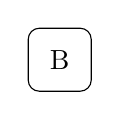
\begin{tikzpicture}
        \node[rounded corners,draw=black,minimum size=0.8cm]{B};
    \end{tikzpicture}
    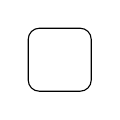
\begin{tikzpicture}
        \node[rounded corners,draw=black,minimum size=0.8cm]{};
    \end{tikzpicture}
    };
     \node[text width=3cm] at (-3,-2.5) 
    {Miss on B as first instance, add B to cache};
    
    \node[rounded corners,draw=black,minimum size=2cm] (c) at (0,-5)  {   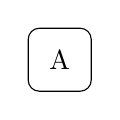
\begin{tikzpicture}
        \node[rounded corners,draw=black,minimum size=0.8cm]{A};
    \end{tikzpicture}
    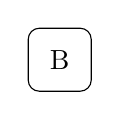
\begin{tikzpicture}
        \node[rounded corners,draw=black,minimum size=0.8cm]{B};
    \end{tikzpicture}
    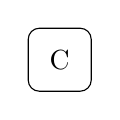
\begin{tikzpicture}
        \node[rounded corners,draw=black,minimum size=0.8cm]{C};
    \end{tikzpicture}
    };

    \node[text width=3cm] at (-3,-5) 
    {Miss on C as first instance, C added to cache};
      
    \node[rounded corners,draw=black,minimum size=2cm] (d) at (0,-7.5)  {   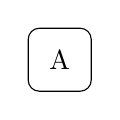
\begin{tikzpicture}
        \node[rounded corners,draw=black,minimum size=0.8cm]{A};
    \end{tikzpicture}
    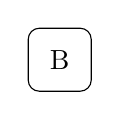
\begin{tikzpicture}
        \node[rounded corners,draw=black,minimum size=0.8cm]{B};
    \end{tikzpicture}
    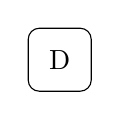
\begin{tikzpicture}
        \node[rounded corners,draw=black,minimum size=0.8cm]{D};
    \end{tikzpicture}
    };

     \node[text width=3cm] at (-3,-7.5) 
    {Miss on D as first instance, evict C since MRU};
    
    \node[rounded corners,draw=black,minimum size=2cm, below left=1 cm of d] (e) at (2.2,-8.4)  { 
    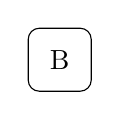
\begin{tikzpicture}
        \node[rounded corners,draw=black,minimum size=0.8cm]{B};
    \end{tikzpicture}
    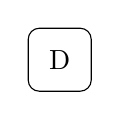
\begin{tikzpicture}
        \node[rounded corners,draw=black,minimum size=0.8cm]{D};
    \end{tikzpicture}
    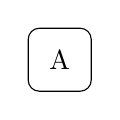
\begin{tikzpicture}
        \node[rounded corners,draw=black,minimum size=0.8cm]{A};
    \end{tikzpicture}
    };  

     \node[text width=3cm] at (-3,-10) 
    {Hit on B};

    \node[rounded corners,draw=black,minimum size=2cm, below left=1 cm of d] (f) at (2.2,-11)  { 
    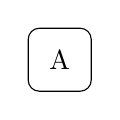
\begin{tikzpicture}
        \node[rounded corners,draw=black,minimum size=0.8cm]{A};
    \end{tikzpicture}
    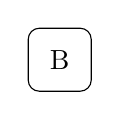
\begin{tikzpicture}
        \node[rounded corners,draw=black,minimum size=0.8cm]{B};
    \end{tikzpicture}
    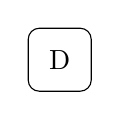
\begin{tikzpicture}
        \node[rounded corners,draw=black,minimum size=0.8cm]{D};
    \end{tikzpicture}
    };  

     \node[text width=3cm] at (-3,-12.5) 
    {Hit on D};

    \node[rounded corners,draw=black,minimum size=2cm, below left=1 cm of d] (g) at (2.2,-13.5)  { 
    \begin{tikzpicture}
        \node[rounded corners,draw=black,minimum size=0.8cm]{A};
    \end{tikzpicture}
    \begin{tikzpicture}
        \node[rounded corners,draw=black,minimum size=0.8cm]{D};
    \end{tikzpicture}
    \begin{tikzpicture}
        \node[rounded corners,draw=black,minimum size=0.8cm]{B};
    \end{tikzpicture}
    };  

     \node[text width=3cm] at (-3,-15) 
    {Hit on A};

    \draw[thick,->] (a) -- (b);
    \draw[thick,->](b) -- (c);  
    \draw[thick,->](c) -- (d);  
    \draw[thick,->](d) -- (e);  
    \draw[thick,->](e) -- (f);  
    \draw[thick,->](f) -- (g);  
\end{tikzpicture}
\end{figure}

\section{Measuring algorithm Performance}
Given these algorithms, one may consider looking at a set of traces to see which algorithm performs better. Let's do this in the paging model with the two traces in Figures 3.2 and 3.3.

On the trace in Figure 3.2, LRU ends up missing less than MRU. As discussed before, we aim to minimize the total number of misses in a cache as they cause the system to slow down. So given this trace and this cache size, we want to choose LRU to maximize performance.

On the trace in Figure 3.3, MRU ends up missing less than LRU. So given this trace and this cache size, we want to choose MRU to maximize performance.

\begin{figure}[h]
    
    \centering
    \caption{How MRU performs against LRU given the trace: A, B, C, D, C}
    \label{fig:my_label}
    \scalebox{.85}{
\begin{tikzpicture} 
    \node[rounded corners,draw=black,label=above:MRU, minimum size=2cm] (a) at (0,0)  {
    \begin{tikzpicture}
        \node[rounded corners,draw=black,minimum size=0.8cm]{A};
    \end{tikzpicture}
    \begin{tikzpicture}
        \node[rounded corners,draw=black,minimum size=0.8cm]{};
    \end{tikzpicture}
    \begin{tikzpicture}
        \node[rounded corners,draw=black,minimum size=0.8cm]{};
    \end{tikzpicture}
    };
    \node[text width=3cm] at (-3, 0) 
    {Miss on A, A added to cache};

    
    \node[rounded corners,draw=black,minimum size=2cm] (b) at (0,-2.5)  {   \begin{tikzpicture}
        \node[rounded corners,draw=black,minimum size=0.8cm]{A};
    \end{tikzpicture}
    \begin{tikzpicture}
        \node[rounded corners,draw=black,minimum size=0.8cm]{B};
    \end{tikzpicture}
    \begin{tikzpicture}
        \node[rounded corners,draw=black,minimum size=0.8cm]{};
    \end{tikzpicture}
    };
     \node[text width=3cm] at (-3,-2.5) 
    {Miss on B, B added to cache};
    
    \node[rounded corners,draw=black,minimum size=2cm] (c) at (0,-5)  {   \begin{tikzpicture}
        \node[rounded corners,draw=black,minimum size=0.8cm]{A};
    \end{tikzpicture}
    \begin{tikzpicture}
        \node[rounded corners,draw=black,minimum size=0.8cm]{B};
    \end{tikzpicture}
    \begin{tikzpicture}
        \node[rounded corners,draw=black,minimum size=0.8cm]{C};
    \end{tikzpicture}
    };

    \node[text width=3cm] at (-3,-5) 
    {Miss on C, C added to cache};
      
    \node[rounded corners,draw=black,minimum size=2cm] (d) at (0,-7.5)  {   \begin{tikzpicture}
        \node[rounded corners,draw=black,minimum size=0.8cm]{A};
    \end{tikzpicture}
    \begin{tikzpicture}
        \node[rounded corners,draw=black,minimum size=0.8cm]{B};
    \end{tikzpicture}
    \begin{tikzpicture}
        \node[rounded corners,draw=black,minimum size=0.8cm]{D};
    \end{tikzpicture}
    };

     \node[text width=3cm] at (-3,-7.5) 
    {Miss on D, D added to cache, evict C since MRU};
    
    \node[rounded corners,draw=black,minimum size=2cm, below left=1 cm of d] (e) at (2.2,-8.4)  { 
    \begin{tikzpicture}
        \node[rounded corners,draw=black,minimum size=0.8cm]{A};
    \end{tikzpicture}
    \begin{tikzpicture}
        \node[rounded corners,draw=black,minimum size=0.8cm]{B};
    \end{tikzpicture}
    \begin{tikzpicture}
        \node[rounded corners,draw=black,minimum size=0.8cm]{C};
    \end{tikzpicture}
    };  

     \node[text width=2.5cm] at (-2.5,-9.8) 
    {Miss on C, evict D since MRU};
















    %LRU
    \node[rounded corners,draw=black,label=above:LRU, minimum size=2cm] (i) at (6,0)  {
    \begin{tikzpicture}
        \node[rounded corners,draw=black,minimum size=0.8cm]{A};
    \end{tikzpicture}
    \begin{tikzpicture}
        \node[rounded corners,draw=black,minimum size=0.8cm]{};
    \end{tikzpicture}
    \begin{tikzpicture}
        \node[rounded corners,draw=black,minimum size=0.8cm]{};
    \end{tikzpicture}
    };
    \node[text width=3cm] at (10,0) 
    {Miss on A, A added to cache};
    \node[text width=3cm] at (4,0) 
    {\Huge A};

    
    \node[rounded corners,draw=black,minimum size=2cm] (j) at (6,-2.5)  {   \begin{tikzpicture}
        \node[rounded corners,draw=black,minimum size=0.8cm]{A};
    \end{tikzpicture}
    \begin{tikzpicture}
        \node[rounded corners,draw=black,minimum size=0.8cm]{B};
    \end{tikzpicture}
    \begin{tikzpicture}
        \node[rounded corners,draw=black,minimum size=0.8cm]{};
    \end{tikzpicture}
    };
    \node[text width=3cm] at (10,-2.4) 
    {Miss on B, B added to cache};
    \node[text width=3cm] at (4,-2.4) 
    {\Huge B};
    
    \node[rounded corners,draw=black,minimum size=2cm] (k) at (6,-5)  {   \begin{tikzpicture}
        \node[rounded corners,draw=black,minimum size=0.8cm]{A};
    \end{tikzpicture}
    \begin{tikzpicture}
        \node[rounded corners,draw=black,minimum size=0.8cm]{B};
    \end{tikzpicture}
    \begin{tikzpicture}
        \node[rounded corners,draw=black,minimum size=0.8cm]{C};
    \end{tikzpicture}
    };
    \node[text width=3cm] at (10,-4.8) 
    {Miss on C, C added to cache};
    \node[text width=3cm] at (4,-4.8) 
    {\Huge C};
    
      
    \node[rounded corners,draw=black,minimum size=2cm] (l) at (6,-7.5)  {   \begin{tikzpicture}
        \node[rounded corners,draw=black,minimum size=0.8cm]{D};
    \end{tikzpicture}
    \begin{tikzpicture}
        \node[rounded corners,draw=black,minimum size=0.8cm]{B};
    \end{tikzpicture}
    \begin{tikzpicture}
        \node[rounded corners,draw=black,minimum size=0.8cm]{C};
    \end{tikzpicture}
    };
     \node[text width=3cm] at (10,-7.4) 
    {Miss on D, D added to cache, Evict A since LRU};
    \node[text width=3cm] at (4,-7.4) 
    {\Huge D};

    
    \node[rounded corners,draw=black,minimum size=2cm, below left=1 cm of l] (m) at (8.2,-8.4)  { 
    \begin{tikzpicture}
        \node[rounded corners,draw=black,minimum size=0.8cm]{D};
    \end{tikzpicture}
    \begin{tikzpicture}
        \node[rounded corners,draw=black,minimum size=0.8cm]{A};
    \end{tikzpicture}
    \begin{tikzpicture}
        \node[rounded corners,draw=black,minimum size=0.8cm]{C};
    \end{tikzpicture}
    };  
    \node[text width=3cm] at (10,-10) 
    {Hit on C};
    \node[text width=3cm] at (4,-10) 
    {\Huge C};


    \draw[thick,->] (a) -- (b);
    \draw[thick,->](b) -- (c);  
    \draw[thick,->](c) -- (d);  
    \draw[thick,->](d) -- (e);  

    
    \draw[thick,->] (i) -- (j);
    \draw[thick,->](j) -- (k);  
    \draw[thick,->](k) -- (l);  
    \draw[thick,->](l) -- (m);  
\end{tikzpicture}
}
\end{figure}
\hfill \break
\hfill \break
\hfill \break
\hfill \break
\hfill \break
\hfill \break
\hfill \break
\hfill \break

\begin{figure}[H]
    \centering
    \caption{How MRU performs against LRU given the trace: A, B, C, D, A}
    \label{fig:my_label}
\scalebox{.85}{
    \begin{tikzpicture} 
    \node[rounded corners,draw=black,label=above:MRU, minimum size=2cm] (a) at (0,0)  {
    \begin{tikzpicture}
        \node[rounded corners,draw=black,minimum size=0.8cm]{A};
    \end{tikzpicture}
    \begin{tikzpicture}
        \node[rounded corners,draw=black,minimum size=0.8cm]{};
    \end{tikzpicture}
    \begin{tikzpicture}
        \node[rounded corners,draw=black,minimum size=0.8cm]{};
    \end{tikzpicture}
    };
    \node[text width=3cm] at (-3, 0) 
    {Miss on A, A added to cache};

    
    \node[rounded corners,draw=black,minimum size=2cm] (b) at (0,-2.5)  {   \begin{tikzpicture}
        \node[rounded corners,draw=black,minimum size=0.8cm]{A};
    \end{tikzpicture}
    \begin{tikzpicture}
        \node[rounded corners,draw=black,minimum size=0.8cm]{B};
    \end{tikzpicture}
    \begin{tikzpicture}
        \node[rounded corners,draw=black,minimum size=0.8cm]{};
    \end{tikzpicture}
    };
     \node[text width=3cm] at (-3,-2.5) 
    {Miss on B, B added to cache};
    
    \node[rounded corners,draw=black,minimum size=2cm] (c) at (0,-5)  {   \begin{tikzpicture}
        \node[rounded corners,draw=black,minimum size=0.8cm]{A};
    \end{tikzpicture}
    \begin{tikzpicture}
        \node[rounded corners,draw=black,minimum size=0.8cm]{B};
    \end{tikzpicture}
    \begin{tikzpicture}
        \node[rounded corners,draw=black,minimum size=0.8cm]{C};
    \end{tikzpicture}
    };

    \node[text width=3cm] at (-3,-5) 
    {Miss on C, C added to cache};
      
    \node[rounded corners,draw=black,minimum size=2cm] (d) at (0,-7.5)  {   \begin{tikzpicture}
        \node[rounded corners,draw=black,minimum size=0.8cm]{A};
    \end{tikzpicture}
    \begin{tikzpicture}
        \node[rounded corners,draw=black,minimum size=0.8cm]{B};
    \end{tikzpicture}
    \begin{tikzpicture}
        \node[rounded corners,draw=black,minimum size=0.8cm]{D};
    \end{tikzpicture}
    };

     \node[text width=3cm] at (-3,-7.5) 
    {Miss on D, add D to cache, evict C since MRU};
    
    \node[rounded corners,draw=black,minimum size=2cm, below left=1 cm of d] (e) at (2.2,-8.4)  { 
    \begin{tikzpicture}
        \node[rounded corners,draw=black,minimum size=0.8cm]{A};
    \end{tikzpicture}
    \begin{tikzpicture}
        \node[rounded corners,draw=black,minimum size=0.8cm]{B};
    \end{tikzpicture}
    \begin{tikzpicture}
        \node[rounded corners,draw=black,minimum size=0.8cm]{C};
    \end{tikzpicture}
    };  

     \node[text width=2.5cm] at (-2.5,-9.8) 
    {Hit on A};
















    %LRU
    \node[rounded corners,draw=black,label=above:LRU, minimum size=2cm] (i) at (6,0)  {
    \begin{tikzpicture}
        \node[rounded corners,draw=black,minimum size=0.8cm]{A};
    \end{tikzpicture}
    \begin{tikzpicture}
        \node[rounded corners,draw=black,minimum size=0.8cm]{};
    \end{tikzpicture}
    \begin{tikzpicture}
        \node[rounded corners,draw=black,minimum size=0.8cm]{};
    \end{tikzpicture}
    };
    \node[text width=3cm] at (10,0) 
    {Miss on A, A added to cache};
    \node[text width=3cm] at (4,0) 
    {\Huge A};

    
    \node[rounded corners,draw=black,minimum size=2cm] (j) at (6,-2.5)  {   \begin{tikzpicture}
        \node[rounded corners,draw=black,minimum size=0.8cm]{A};
    \end{tikzpicture}
    \begin{tikzpicture}
        \node[rounded corners,draw=black,minimum size=0.8cm]{B};
    \end{tikzpicture}
    \begin{tikzpicture}
        \node[rounded corners,draw=black,minimum size=0.8cm]{};
    \end{tikzpicture}
    };
    \node[text width=3cm] at (10,-2.4) 
    {Miss on B, B added to cache};
    \node[text width=3cm] at (4,-2.4) 
    {\Huge B};
    
    \node[rounded corners,draw=black,minimum size=2cm] (k) at (6,-5)  {   \begin{tikzpicture}
        \node[rounded corners,draw=black,minimum size=0.8cm]{A};
    \end{tikzpicture}
    \begin{tikzpicture}
        \node[rounded corners,draw=black,minimum size=0.8cm]{B};
    \end{tikzpicture}
    \begin{tikzpicture}
        \node[rounded corners,draw=black,minimum size=0.8cm]{C};
    \end{tikzpicture}
    };
    \node[text width=3cm] at (10,-4.8) 
    {Miss on C, C added to cache};
    \node[text width=3cm] at (4,-4.8) 
    {\Huge C};
    
      
    \node[rounded corners,draw=black,minimum size=2cm] (l) at (6,-7.5)  {   \begin{tikzpicture}
        \node[rounded corners,draw=black,minimum size=0.8cm]{D};
    \end{tikzpicture}
    \begin{tikzpicture}
        \node[rounded corners,draw=black,minimum size=0.8cm]{B};
    \end{tikzpicture}
    \begin{tikzpicture}
        \node[rounded corners,draw=black,minimum size=0.8cm]{C};
    \end{tikzpicture}
    };
     \node[text width=3cm] at (10,-7.4) 
    {Miss on D, D added to cache, Evict A since LRU};
    \node[text width=3cm] at (4,-7.4) 
    {\Huge D};

    
    \node[rounded corners,draw=black,minimum size=2cm, below left=1 cm of l] (m) at (8.2,-8.4)  { 
    \begin{tikzpicture}
        \node[rounded corners,draw=black,minimum size=0.8cm]{D};
    \end{tikzpicture}
    \begin{tikzpicture}
        \node[rounded corners,draw=black,minimum size=0.8cm]{A};
    \end{tikzpicture}
    \begin{tikzpicture}
        \node[rounded corners,draw=black,minimum size=0.8cm]{C};
    \end{tikzpicture}
    };  
    \node[text width=3cm] at (10,-10) 
    {Miss on A, A added to cache, evict B since LRU};
    \node[text width=3cm] at (4,-10) 
    {\Huge A};


    \draw[thick,->] (a) -- (b);
    \draw[thick,->](b) -- (c);  
    \draw[thick,->](c) -- (d);  
    \draw[thick,->](d) -- (e);  

    
    \draw[thick,->] (i) -- (j);
    \draw[thick,->](j) -- (k);  
    \draw[thick,->](k) -- (l);  
    \draw[thick,->](l) -- (m);  
\end{tikzpicture}
}
\end{figure}

Does the fact that these algorithms perform differently on these traces mean that comparison of algorithms on traces is not a useful metric? No. These traces are what are called adversarial traces, meaning that they are specifically made to make an algorithm perform as badly as it possibly can. So trace 1 in Figure 3.2 is made specifically to perform poorly with MRU. If this trace were to be repeated, MRU would begin to miss every item. The same is true of LRU in the trace from Figure 3.3.

These adversarial traces pose a challenge, as there will almost always be a way to structure a trace so that any algorithm A has maximal misses. Even looking at how they perform over a large set of traces does not give much insight, as there are infinitely many traces that can be tested. So instead of looking at comparing these algorithms on any specific trace or set of traces, we instead seek to look to create a more even playing field for these algorithms' performance to be judged.
\hfill \break
\hfill \break
\hfill \break
\hfill \break
\hfill \break


\section{Competitive Ratios}
Competitive ratios are the ways that we can bound the performance of an algorithm more fairly than by testing directly on traces. These ratios are theoretical, meaning they are a good measurement of how algorithms perform in the abstract.

Now to find these competitive ratios, we compare algorithm A to algorithm B. Specifically, given $\sigma$ so that algorithm B performs with minimum misses on the trace. Then we compare the number of misses they both have, giving us that competitive ratio of $\frac{misses(A)}{misses(B)}$. The question then becomes: how does one decide this B so that it has minimal misses? This is done through the use of an optimal algorithm.

\subsection{Optimal Algorithms}
Offline algorithms are a class of algorithms used in computer science that operate using information about an entire trace to make decisions rather than processing data as it arrives a request at a time. Optimal algorithms are then required to be offline to minimize misses as they need to see the entire trace to make eviction decisions. The algorithms we have discussed so far have all been Online algorithms, meaning they process items 1 request at a time and can only make decisions based on current and past requests. 

This distinction between these online and offline algorithms means that optimal algorithms have the entirety of the input data available in advance, and can take as much time and memory as needed to produce the output with the least number of misses in the paging model. This trait means we can then use them to bind how an algorithm performs as they always perform with these minimal number of misses. 

OPT works in the paging model by, when needing to evict an item, finding the item that is furthest in the future. This is because the item furthest in the future has the

Figure 3.4 is an example of how OPT uses its knowledge of the entire trace to make minimal misses when compared to LRU. In this trace, OPT only misses on the first instance of an item and manages to hit on all others, while LRU manages to miss on the last A and B as well as all items OPT misses. This is because OPT can process the entire trace before making any decisions and can then keep misses minimal. 

Now that there is this OPT algorithm that we can compare other algorithms to, we want to see what the best performance case is for algorithm A when compared to OPT. We want to do this because OPT always performs the best any algorithm can on a trace. This means that when compared to OPT, all other algorithms are put onto the same playing field.


\hfill \break
\hfill \break
\hfill \break
\hfill \break
\hfill \break
\hfill \break
\hfill \break
\hfill \break
\hfill \break
\hfill \break


\begin{figure}[H]
    \centering
    \caption{How OPT performs when compared to an online algorithm LRU given the trace: A, B, C, D, A, B, C, C}
    \label{fig:my_label}
\begin{tikzpicture} 
    \node[rounded corners,draw=black,label=above:OPT, minimum size=2cm] (a) at (0,0)  {
    \begin{tikzpicture}
        \node[rounded corners,draw=black,minimum size=0.8cm]{A};
    \end{tikzpicture}
    \begin{tikzpicture}
        \node[rounded corners,draw=black,minimum size=0.8cm]{};
    \end{tikzpicture}
    \begin{tikzpicture}
        \node[rounded corners,draw=black,minimum size=0.8cm]{};
    \end{tikzpicture}
    };
    \node[text width=3cm] at (-3, 0) 
    {Miss on A, A added to cache};

    
    \node[rounded corners,draw=black,minimum size=2cm] (b) at (0,-2.5)  {   \begin{tikzpicture}
        \node[rounded corners,draw=black,minimum size=0.8cm]{A};
    \end{tikzpicture}
    \begin{tikzpicture}
        \node[rounded corners,draw=black,minimum size=0.8cm]{B};
    \end{tikzpicture}
    \begin{tikzpicture}
        \node[rounded corners,draw=black,minimum size=0.8cm]{};
    \end{tikzpicture}
    };
     \node[text width=3cm] at (-3,-2.5) 
    {Miss on B, B added to cache};
    
    \node[rounded corners,draw=black,minimum size=2cm] (c) at (0,-5)  {   \begin{tikzpicture}
        \node[rounded corners,draw=black,minimum size=0.8cm]{A};
    \end{tikzpicture}
    \begin{tikzpicture}
        \node[rounded corners,draw=black,minimum size=0.8cm]{B};
    \end{tikzpicture}
    \begin{tikzpicture}
        \node[rounded corners,draw=black,minimum size=0.8cm]{C};
    \end{tikzpicture}
    };

    \node[text width=3cm] at (-3,-5) 
    {Miss on C, C added to cache};
      
    \node[rounded corners,draw=black,minimum size=2cm] (d) at (0,-7.5)  {   \begin{tikzpicture}
        \node[rounded corners,draw=black,minimum size=0.8cm]{A};
    \end{tikzpicture}
    \begin{tikzpicture}
        \node[rounded corners,draw=black,minimum size=0.8cm]{B};
    \end{tikzpicture}
    \begin{tikzpicture}
        \node[rounded corners,draw=black,minimum size=0.8cm]{D};
    \end{tikzpicture}
    };

     \node[text width=3cm] at (-3,-7.5) 
    {Miss on D, D added to cache, evict C since FITF};
    
    \node[rounded corners,draw=black,minimum size=2cm, below left=1 cm of d] (e) at (2.2,-8.4)  { 
    \begin{tikzpicture}
        \node[rounded corners,draw=black,minimum size=0.8cm]{A};
    \end{tikzpicture}
    \begin{tikzpicture}
        \node[rounded corners,draw=black,minimum size=0.8cm]{B};
    \end{tikzpicture}
    \begin{tikzpicture}
        \node[rounded corners,draw=black,minimum size=0.8cm]{D};
    \end{tikzpicture}
    };  

     \node[text width=3cm] at (-2.5,-9.8) 
    {Hit on A};
    
    \node[rounded corners,draw=black,minimum size=2cm,below left=1 cm of e] (f) at (2.2,-10.8)  { 
    \begin{tikzpicture}
        \node[rounded corners,draw=black,minimum size=0.8cm]{A};
    \end{tikzpicture}
    \begin{tikzpicture}
        \node[rounded corners,draw=black,minimum size=0.8cm]{B};
    \end{tikzpicture}
    \begin{tikzpicture}
        \node[rounded corners,draw=black,minimum size=0.8cm]{D};
    \end{tikzpicture}
    };  

     \node[text width=3cm] at (-2.5,-12.2) 
    {Hit on B};

    
    \node[rounded corners,draw=black,minimum size=2cm, below left=1 cm of f] (g) at (2.2,-13.4)  { 
    \begin{tikzpicture}
        \node[rounded corners,draw=black,minimum size=0.8cm]{A};
    \end{tikzpicture}
    \begin{tikzpicture}
        \node[rounded corners,draw=black,minimum size=0.8cm]{B};
    \end{tikzpicture}
    \begin{tikzpicture}
        \node[rounded corners,draw=black,minimum size=0.8cm]{D};
    \end{tikzpicture}
    };  

     \node[text width=3cm] at (-3,-14.7) 
    {Miss on C, evict D};
    
    \node[rounded corners,draw=black,minimum size=2cm, below left=1 cm of g] (h) at (2.2,-15.6)  { 
    \begin{tikzpicture}
        \node[rounded corners,draw=black,minimum size=0.8cm]{A};
    \end{tikzpicture}
    \begin{tikzpicture}
        \node[rounded corners,draw=black,minimum size=0.8cm]{B};
    \end{tikzpicture}
    \begin{tikzpicture}
        \node[rounded corners,draw=black,minimum size=0.8cm]{C};
    \end{tikzpicture}
    }; 
    \node[text width=3cm] at (-2.5,-17.3) 
    {Hit on C};






















    %LRU
    \node[rounded corners,draw=black,label=above:LRU, minimum size=2cm] (i) at (6,0)  {
    \begin{tikzpicture}
        \node[rounded corners,draw=black,minimum size=0.8cm]{A};
    \end{tikzpicture}
    \begin{tikzpicture}
        \node[rounded corners,draw=black,minimum size=0.8cm]{};
    \end{tikzpicture}
    \begin{tikzpicture}
        \node[rounded corners,draw=black,minimum size=0.8cm]{};
    \end{tikzpicture}
    };
    \node[text width=3cm] at (10,0) 
    {Miss on A, A added to cache};
    \node[text width=3cm] at (4,0) 
    {\Huge A};

    
    \node[rounded corners,draw=black,minimum size=2cm] (j) at (6,-2.5)  {   \begin{tikzpicture}
        \node[rounded corners,draw=black,minimum size=0.8cm]{A};
    \end{tikzpicture}
    \begin{tikzpicture}
        \node[rounded corners,draw=black,minimum size=0.8cm]{B};
    \end{tikzpicture}
    \begin{tikzpicture}
        \node[rounded corners,draw=black,minimum size=0.8cm]{};
    \end{tikzpicture}
    };
    \node[text width=3cm] at (10,-2.4) 
    {Miss on B, B added to cache};
    \node[text width=3cm] at (4,-2.4) 
    {\Huge B};
    
    \node[rounded corners,draw=black,minimum size=2cm] (k) at (6,-5)  {   \begin{tikzpicture}
        \node[rounded corners,draw=black,minimum size=0.8cm]{A};
    \end{tikzpicture}
    \begin{tikzpicture}
        \node[rounded corners,draw=black,minimum size=0.8cm]{B};
    \end{tikzpicture}
    \begin{tikzpicture}
        \node[rounded corners,draw=black,minimum size=0.8cm]{C};
    \end{tikzpicture}
    };
    \node[text width=3cm] at (10,-4.8) 
    {Miss on C, C added to cache};
    \node[text width=3cm] at (4,-4.8) 
    {\Huge C};
    
      
    \node[rounded corners,draw=black,minimum size=2cm] (l) at (6,-7.5)  {   \begin{tikzpicture}
        \node[rounded corners,draw=black,minimum size=0.8cm]{D};
    \end{tikzpicture}
    \begin{tikzpicture}
        \node[rounded corners,draw=black,minimum size=0.8cm]{B};
    \end{tikzpicture}
    \begin{tikzpicture}
        \node[rounded corners,draw=black,minimum size=0.8cm]{C};
    \end{tikzpicture}
    };
     \node[text width=3cm] at (10,-7.4) 
    {Miss on D, Evict A as LRU};
    \node[text width=3cm] at (4,-7.4) 
    {\Huge D};

    
    \node[rounded corners,draw=black,minimum size=2cm, below left=1 cm of l] (m) at (8.2,-8.4)  { 
    \begin{tikzpicture}
        \node[rounded corners,draw=black,minimum size=0.8cm]{D};
    \end{tikzpicture}
    \begin{tikzpicture}
        \node[rounded corners,draw=black,minimum size=0.8cm]{A};
    \end{tikzpicture}
    \begin{tikzpicture}
        \node[rounded corners,draw=black,minimum size=0.8cm]{C};
    \end{tikzpicture}
    };  
    \node[text width=3cm] at (10,-10) 
    {Miss on A, Evict B since LRU};
    \node[text width=3cm] at (4,-10) 
    {\Huge A};

    
    \node[rounded corners,draw=black,minimum size=2cm,below left=1 cm of m] (n) at (8.2,-10.8)  { 
    \begin{tikzpicture}
        \node[rounded corners,draw=black,minimum size=0.8cm]{D};
    \end{tikzpicture}
    \begin{tikzpicture}
        \node[rounded corners,draw=black,minimum size=0.8cm]{A};
    \end{tikzpicture}
    \begin{tikzpicture}
        \node[rounded corners,draw=black,minimum size=0.8cm]{B};
    \end{tikzpicture}
    };  
     \node[text width=3cm] at (10,-12.3) 
    {Miss on B, Evict C since LRU};
    \node[text width=3cm] at (4,-12.3) 
    {\Huge B};

    
    \node[rounded corners,draw=black,minimum size=2cm, below left=1 cm of n] (o) at (8.2,-13.4)  { 
    \begin{tikzpicture}
        \node[rounded corners,draw=black,minimum size=0.8cm]{C};
    \end{tikzpicture}
    \begin{tikzpicture}
        \node[rounded corners,draw=black,minimum size=0.8cm]{A};
    \end{tikzpicture}
    \begin{tikzpicture}
        \node[rounded corners,draw=black,minimum size=0.8cm]{B};
    \end{tikzpicture}
    };  
    \node[text width=3cm] at (10,-14.8) 
    {Miss on C, evict B};
    \node[text width=3cm] at (4,-14.8) 
    {\Huge C};
    
    
    \node[rounded corners,draw=black,minimum size=2cm, below left=1 cm of o] (p) at (8.2,-15.6)  { 
    \begin{tikzpicture}
        \node[rounded corners,draw=black,minimum size=0.8cm]{C};
    \end{tikzpicture}
    \begin{tikzpicture}
        \node[rounded corners,draw=black,minimum size=0.8cm]{A};
    \end{tikzpicture}
    \begin{tikzpicture}
        \node[rounded corners,draw=black,minimum size=0.8cm]{B};
    \end{tikzpicture}
    };  
    \node[text width=3cm] at (10,-17.3) 
    {Hit on C};
    \node[text width=3cm] at (4,-17.3) 
    {\Huge C};

    \draw[thick,->] (a) -- (b);
    \draw[thick,->](b) -- (c);  
    \draw[thick,->](c) -- (d);  
    \draw[thick,->](d) -- (e);  
    \draw[thick,->] (e) -- (f);
    \draw[thick,->](f) -- (g);  
    \draw[thick,->](g) -- (h);
    
    \draw[thick,->] (i) -- (j);
    \draw[thick,->](j) -- (k);  
    \draw[thick,->](k) -- (l);  
    \draw[thick,->](l) -- (m);  
    \draw[thick,->] (m) -- (n);
    \draw[thick,->](n) -- (o);  
    \draw[thick,->](o) -- (p);
        
\end{tikzpicture}
\end{figure}

\subsection{Competitive Lower Bounds}
The lower competitive bound refers to the minimum ratio of misses any algorithm A can have when compared to OPT.

The minimum competitive bound for algorithms was first established by Sleator and Tarjan in their paper "Amortized efficiency of list update and paging rules" in 1985. They proved that the lower competitive bound of all deterministic algorithms when compared to OPT is $\frac{k}{k-h+1}$ \cite{sleator1985amortized}. Where $h$ is the size of OPTs cache and $k$ is the size of the algorithms cache.

This result from Sleator and Tarjan shows that no algorithm processing a trace one request at a time can achieve a competitive ratio better than $\frac{k}{k-h+1}$, regardless of its design or implementation. As a result, much of the research in caching algorithms has focused on developing algorithms that can achieve competitive ratios that are close to or equal to this lower bound.

This alone doesn't mean that algorithms always perform this poorly when compared to OPT as it is just a lower bound for how well it can do. Instead, when looking to see how an algorithm performs, we also look to see what its upper bounds are.



\section{Upper Bounds}
The upper competitive bound refers to the maximum competitive ratio that any algorithm can achieve relative to OPT, and unlike competitive lower bounds, there is no maximum upper bound. This means that there is no maximum cost ratio that an algorithm can pay when compared to OPT.

This means that algorithms are designed to have upper bounds to be as close to the minimal lower bound $\frac{k}{k-h+1}$ as possible. If an algorithm achieves this upper bound, it would mean that its bounded competitive ratio is $\frac{k}{k-h+1}$. For an algorithm to have these matching bounds, it would mean that it performs as well as any algorithm can when compared to OPT.

LRU was shown in \cite{sleator1985amortized} to have these matching lower and upper bounds in the paging model. This means that LRU performs competitively to the minimum bounds of online caching algorithms in any circumstance in the paging model.
MRU was then shown \cite{agrawal2007worst} to have no maximum upper bound, this means that while MRU may have the same lower bound as LRU, it is possible to pay arbitrarily high cost when compared to OPT. So while LRU always will perform within this $\frac{k}{k-h+1}$ bound, MRU can reach this bound but could pay a much higher ratio.


\hfill \break
\hfill \break
\hfill \break


\section{Landlord}
The landlord algorithm was just one of a set of algorithms that Neal E. Young proposed in \cite{young1994k}. Landlord was created by Young to generalize LRU to the general model as it was limited to the paging model at the time. 

\makeatletter
\def\BState{\State\hskip-\ALG@thistlm}
\makeatother
\algnewcommand\algorithmicforeach{\textbf{for each}}
\algdef{S}[FOR]{ForEach}[1]{\algorithmicforeach\ #1\ \algorithmicdo}




    \begin{algorithm}
\caption{Landlord}\label{euclid}
    \begin{algorithmic}[1]
    \BState \emph{loop}:
        \State $\textit{Item} \gets \text{nextItem in trace}$
        \If {$\textit{Item} \text{ not in Cache}$}
            \While{$\text{Cache can't contain Item}$}
                \State $x \gets y\in cache \text{ with } min(\frac{cost(y)}{size(y)})$
                    \State $\Delta \gets \frac{credit(x)}{size(x)}$
                    \ForEach {$f \in cache $}
                        \State $credit(f) \gets credit(f) - \Delta \times size(f)$
                    \EndFor
                    \State $\exists f, credit(f)=0,\text{ Evict(f)} $        \EndWhile
            \State $credit(Item) \gets cost(Item)$
        \Else 
         \State $credit(i) \gets \text{value between current credit and cost}$
        \EndIf
    \end{algorithmic}
\end{algorithm}




As can be seen in this pseudo code, Landlord gives each item a credit C when it enters the cache from memory. This credit C is always positive as it is an estimation of how much you want this specific item in a cache.

When a replacement decision is made in Landlord, the items with 0 credit value are evicted. As requests get processed, the credit of all items in the cache gets reduced by a function of the lowest priority item's cost and size and the size of the item itself.

An important thing to note about Landlord is that if an item is already in the cache and is accessed again, its credit is reset to some number between an item's current credit and its max credit. This then allows items that are in the cache and accessed frequently to always have more credit than those in the cache that is accessed infrequently. This structure of credit renewal allows the algorithm to take advantage of the temporal locality of accesses.

Figure 3.5 shows how Landlord functions on an example trace and explains why it makes the evictions it does.


\begin{figure}[h]
    \centering
    \caption{Landlord's Performance on a trace}
    \label{fig:my_label}
Given cache size 3 and the trace: A,B,C,D,B,C,C,B with item costs 40,4,8,2 and size 1
\begin{tikzpicture}
\node[rounded corners, draw=black,label=above:Priorities, minimum width=5 cm](pri1) at (-8,0){
\begin{tikzpicture}
\node[rounded corners, draw=black, minimum width = 1cm](he){
a $=$ 40
};
\end{tikzpicture}
};
\node[rounded corners, text width = 4cm, left = 0 cm of pri1]{
Item a is given its cost as priority since space in cache
};

\node[rounded corners, draw=black, minimum width=5 cm](pri2) at (-8,-2.5){
\begin{tikzpicture}
\node[rounded corners, draw=black, minimum width = 1cm](he1){
a $=$ 36
};
\node[rounded corners, draw=black, minimum width = 1cm, left = .3cm of he1](he2){
b $=$ 4
};
\end{tikzpicture}

};
\node[rounded corners, text width = 4cm, left = 0 cm of pri2]{
Item b is given its cost as priority since space in cache, decrease A
};


\node[rounded corners, draw=black, minimum width=5 cm](pri3) at (-8,-5.2){
\begin{tikzpicture}
\node[rounded corners, draw=black, minimum width = 1cm](he1){
a $=$ 32
};
\node[rounded corners, draw=black, minimum width = 1cm, left = .3cm of he1](he2){
b $=$ 0
};
\node[rounded corners, draw=black, minimum width = 1cm, left = .3cm of he2](he3){
c $=$ 8
};
\end{tikzpicture}

};
\node[rounded corners, text width = 4cm, left = 0 cm of pri3]{
Item c is given its cost as priority since space in cache, decrease A and B
};

\node[rounded corners, draw=black, minimum width=5 cm](pri4) at (-8,-7.4){
\begin{tikzpicture}
\node[rounded corners, draw=black, minimum width = 1cm](he1){
d $=$ 2
};
\node[rounded corners, draw=black, minimum width = 1cm, left = .3cm of he1](he2){
a $=$ 30
};
\node[rounded corners, draw=black, minimum width = 1cm, left = .3cm of he2](he3){
c $=$ 4
};
\end{tikzpicture}


};
\node[rounded corners, text width = 4cm, left = 0 cm of pri4]{
no room for d, items in cache have priority decreased by $\Delta$ and B evicted
};

\node[rounded corners, draw=black, minimum width=5 cm](pri5) at (-8,-10){
\begin{tikzpicture}
\node[rounded corners, draw=black, minimum width = 1cm](he1){
b $=$ 4
};
\node[rounded corners, draw=black, minimum width = 1cm, left = .3cm of he1](he2){
a $=$ 26
};
\node[rounded corners, draw=black, minimum width = 1cm, left = .3cm of he2](he3){
c $=$ 0
};
\end{tikzpicture}

};

\node[rounded corners, text width = 4cm, left = 0 cm of pri5]{
B credit reset and others decreased by $\Delta$
};

\node[rounded corners, draw=black, minimum width=5 cm](pri6) at (-8,-12.3){
\begin{tikzpicture}
\node[rounded corners, draw=black, minimum width = 1cm, left = .3cm of he1](he2){
a $=$ 18
};
\node[rounded corners, draw=black, minimum width = 1cm, left = .3cm of he2](he3){
c $=$ 8
};
\end{tikzpicture}

};
\node[rounded corners, text width = 4cm, left = 0 cm of pri6]{
C credit reset and others decreased by $\Delta$
};


\node[rounded corners, draw=black, minimum width=5 cm](pri7) at (-8,-15){
\begin{tikzpicture}
\node[rounded corners, draw=black, minimum width = 1cm](he2){
a $=$ 10
};
\node[rounded corners, draw=black, minimum width = 1cm, left = .3cm of he2](he3){
c $=$ 8
};
\end{tikzpicture}

};
\node[rounded corners, text width = 4cm, left = 0 cm of pri7]{
C credit reset and others decreased by $\Delta$
};


\node[rounded corners, draw=black, minimum width=5 cm](pri8) at (-8,-17.2){
\begin{tikzpicture}
\node[rounded corners, draw=black, minimum width = 1cm](he1){
b $=$ 4
};
\node[rounded corners, draw=black, minimum width = 1cm, left = .3cm of he1](he2){
a $=$ 6
};
\node[rounded corners, draw=black, minimum width = 1cm, left = .3cm of he2](he3){
c $=$ 8
};
\end{tikzpicture}
};
\node[rounded corners, text width = 4cm, left = 0 cm of pri8]{
B credit reset and others decreased by $\Delta$
};
 
\end{tikzpicture}
   

\end{figure}


Landlord was shown in \cite{young1994k} to have both a lower and upper competitive ratio of $\frac{k}{k-h+1}$ in the general model. This means that Landlord can perform as well as any algorithm can when compared to OPT.

\chapter{Cost Curves}
\section{Cost Curves}
Cost curves are graphs that depict the relationship between cache size and the cost of items missed by a cache on a trace using a specific algorithm. MRCs are commonly used to evaluate caching algorithms' performance and determine the optimal cache size for a particular system.

The curve typically shows a decreasing cost as the cache size increases, indicating, intuitively, that larger caches are more effective at reducing the number of cache misses. However, the curve will eventually reach a point of diminishing returns, where increasing the cache size further does not significantly reduce the mass ratio. This is because the first instance of any item will never be in the cache so they will always miss and cause a performance decrease.

\begin{figure}[H]
    \centering
    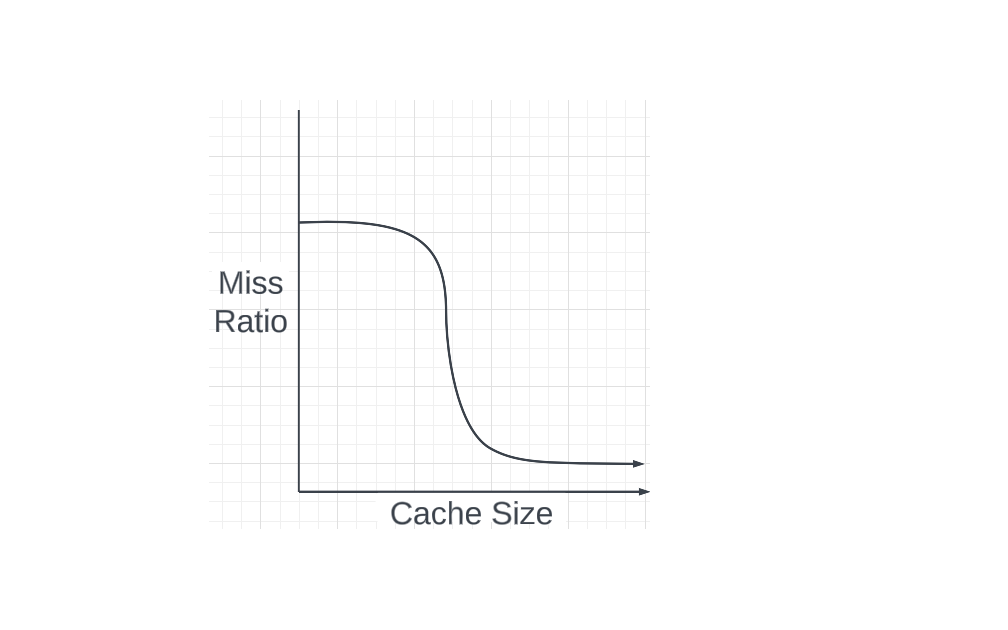
\includegraphics[scale=0.5, trim={.2cm 2.6cm 2.1cm 2.4cm},clip]{thesistemplate_2020-04-24/chapters/MRC shit/mrcFinal.png}
    \caption{Generic MRC}
    \label{fig:my_label}
\end{figure}

Figure 4.1 shows a generalization of what MRCs look like. If a section of the cost curve is almost flat, the cache size is either too large, meaning it misses too little and isn't an efficient use of space, or is too small and isn't gaining the system any efficiency as it misses too often. When designers are creating a cache for a system, they look at this curve and attempt to balance the cost and size to create a cache that improves the system without creating an unnecessary layer of memory.


The naive way to generate these MRCs is to simulate a trace $\sigma$ on all cache sizes with a given algorithm. This requires a large amount of computational effort, as most algorithms when having differing cache sizes make separate choices as to what to evict. An improvement on this method is to only simulate a subset of all cache sizes, but this too is still computationally expensive. There is an important exception to this computationally heavy generation of MRCs, which is to use an algorithm created by \cite{mattson1970evaluation} which allows the generation of an MRC with one pass of the trace $\sigma$.

\section{Mattson's Algorithm}

As stated, the generation of MRCs through running an algorithm on all cache sizes is computationally expensive. Instead, we use an algorithm invented by \cite{mattson1970evaluation} which allows for this generation of MRCs using only $O(nm)$ time where $n$ is the trace length and $m$ is the number of items. Shown here is Mattson's algorithm for LRU in the paging model.


\begin{algorithm}
    \caption{Mattson for LRU}\label{euclid}
        \begin{algorithmic}[1]
            \State $trace = \{i_0 ... i_n \}$
            \For{$x \text{ in range}(0,n) $}
                \State $last\_ Reference = \infty$ \Comment{If an item hasn't been seen before it has $\infty$ priority}
                \For{$z \text{ in range}(x,0) \text{ We go backward in the trace} $}
                    \If {$trace[z] ==trace[x]$} \Comment{trace[x] refers to the item requested}
                        \State $last\_ Reference = z$ \Comment{Update as we have seen the item }
                        \State $\text{Leave Loop}$
                    \EndIf
                \EndFor
                \State $unique\_ Items = \{\}$
                \If{$last\_ Reference \neq \infty$}
                \For{$b \text{ in range}(last\_ Reference,x) $}
                    \If {$trace[b] \text{ not in } unique\_ Items$}
                        \State $\text{push } trace[b] \text{ onto }unique\_ Items$
                    \EndIf
                \EndFor
                \State $Distance = \text{number of items in } unique\_ Items$
                \For{$a \text{ in range}(1,Distance) $}
                    \State $\text{Cost Paid by $cache(a)$}  += cost(trace[x])$ \Comment{cache of size a}
                \EndFor
                \Else 
                    \State $\text{Cost Paid by all cache sizes }  += cost(trace[x])$
                \EndIf
            \EndFor
        \end{algorithmic}
\end{algorithm}

%You don't mention distinctness when you calculate distance, and even if you did, that would still be LRU's stack distance. It's not even accurate for SCP.

When an item $i$ is requested, the number of unique items since the last access is calculated, which is called distance. This distance tells us that all caches with sizes greater than or equal to this number hit on this item as they contain the item in their cache due to LRUs structure. Then all caches with a size less than this number miss on this item and pay its cost as they are too small to still contain the item. In other caching models, when calculating if an item would still be in the cache, you must factor in the size of unique items between repeat requests to the same item, not just the distance in the trace of these requests. 

Here is a generalized version of Mattsons Algorithm
%
\begin{algorithm}
    \caption{Generalized Mattson's for any algorithm}\label{euclid}
        \begin{algorithmic}[1]
            \State $trace = \{i_0 ... i_n \}$
            \State $unique\_ Item\_ Priorities = \{\}$
            \State $unique\_ Items = \{\}$
            \For{$x \text{ in range}(0,n) $}\Comment{trace[x] refers to the item}
                \State $priority = \text{Priority the algorithm assigns to item $trace[x]$ when it is requested}$
                \If {$trace[x] \text{ not in } unique\_ Items$}
                    \State $\text{push } [trace[x],priority] \text{ onto }unique\_ Item\_ Priorities$
                     \State $\text{push } trace[x] \text{ onto }unique\_ Items$
                     \State $\text{Cost Paid by all caches } += cost(trace[x])$
                \Else 
                    \State $size\_Items = 0$
                    \For{$d$ in range $(0,$ (items in $unique\_Item\_ Priorities)$)}
                        \State $size\_ Items+= size(unique\_Item\_ Priorities[d][0])$ \Comment{[d][0] is an item}
                        \If{$unique\_Item\_ Priorities[d][0] == trace[x]$}
                            \State $\text{Cost Paid by all caches of size $<$ $size\_ Items$ } += cost(trace[x])$
                            \State $unique\_Item\_ Priorities[d][1] = priority$             \Comment{update trace[x] priority}
                        \EndIf
                    \EndFor
                \EndIf
                \For{$c \text{ in } unique\_ Item \_Priorities$}
                    \State $currentPriority = c[1]$ \Comment{Which is the current Priority of item c[0]} 
                    \State $change\_ In\_ Priority = 0$             \Comment{An algorithm can choose to alter priority}
                    \If{$\text{request }trace[x]\text{ causes priority change }$}
                        \State $priorityChange =\text{ Priority change of item $c[0]$ from request $trace[x]$}$
                    \EndIf
                    \State $c[1] = currentPriority - newPriority$
                \EndFor
                \State $\text{Reorder $unique\_ Item\_ Priorities$ so item's ordering}$
                \State$\text{in $unique\_ Item\_ Priorities$ goes from highest to lowest priority}$
            \EndFor
        \end{algorithmic}
\end{algorithm}



\begin{algorithm}
    \caption{Generalized Mattson's for any algorithm}\label{euclid}
        \begin{algorithmic}[1]
\State Starting at the beginning of the trace, read the item requests in order and create a priority list of items that starts empty. 
\State For each request, ensure the list is ordered from the item with the highest priority to the item with the lowest priority. 
\State If the item being requested isn't in the priority list, add it to the list with the priority the algorithm assigns and increase the cost paid by all cache sizes by the cost of the item being requested, and move to the next request 
\State Otherwise the item is in the list. Starting from the priority list's beginning, locate the position of the item being requested. As you search for the item, add up the sizes of all items encountered until you find the item being requested. Call this total size d. Then increase the cost paid by all caches of sizes less than d then move to the next request.
\end{algorithmic}
\end{algorithm}


Using this generalized version, you can see that Mattsons algorithm keeps a priority list of all items which is ordered from highest to lowest priority. If an item isn't in this list, all caches must miss and pay its cost. If an item is then in this list, the size of items with priorities greater than the current request's priority is calculated. For all caches that have a size less than this number, they miss and must pay a cost. Then the priorities of all items are updated and reordered, an important note is that some algorithms may not change the priority of an item. This happens in LRU when there are repeated requests to a unique item between requests to the current item, so the item's priorities aren't updated.  
This updating scheme then allows 1 pass of a trace to check all size caches as each request allows the updating of all cache's paid costs. This approach requires that it is limited to a subset of caching algorithms called stack algorithms. 

\subsection{Stack Algorithms}

Stack algorithms are a class of algorithms where: $cache(k) \subseteq cache(k+1)$. This means that all items in $cache(k)$ exist in $cache(k+1)$. This is important as most caching algorithms don't have this structure, this is because their decisions as to what to evict often depend on the size of the cache and the items inside it.

%use diagrams
\begin{figure}[h!]
    \centering
    \caption{How stack algorithms work with differing cache sizes}
    \label{fig:my_label}
\begin{tikzpicture}
 \node[rectangle,draw,  minimum width = 2.9cm, 
    minimum height = 1.1cm, label=above:K-1] (r) at (0,0) {
    };
    \node[rectangle,draw,  minimum width = 3.8cm, 
    minimum height = 2.3cm, label=above:K] (t) at (.4,0) {
    };
    \node[rectangle,draw,  minimum width = 4.8cm, 
    minimum height = 3.3cm, label=above:K+1] (u) at (.9,0) {
    };
    \node[rectangle,draw,  minimum width = 6.2cm, 
    minimum height = 4.5cm, label=above:K+2] (p) at (1.6,0) {
    };
\node[rectangle,draw, minimum width = 4cm, 
    minimum height = 1cm,below right = -0.5cm and -1.5cm of r] (q) at (0,0) {
    \begin{tikzpicture}
            \node[rounded corners,draw=black,minimum size=0.8cm]{a};
    \end{tikzpicture}
    \begin{tikzpicture}
        \node[rounded corners,draw=black,minimum size=0.8cm]{b};
    \end{tikzpicture}
    \begin{tikzpicture}
        \node[rounded corners,draw=black,minimum size=0.8cm]{d};
    \end{tikzpicture}
    \begin{tikzpicture}
        \node[rounded corners,draw=black, minimum size=0.8cm]{e};
    \end{tikzpicture}
    \begin{tikzpicture}
            \node[rounded corners,draw=black,minimum size=0.8cm]{f};
    \end{tikzpicture}
    \begin{tikzpicture}
        \node[rounded corners,draw=black,minimum size=0.8cm]{g};
    \end{tikzpicture}
    };
\end{tikzpicture}
\end{figure}
%\begin{figure}
    \centering
    \caption{Size k=3 cache vs k=4 cache in stack algorithm }
    \label{fig:my_label}
\begin{tikzpicture}


    \node[rounded corners,draw=black,label=above:K, minimum size=2cm] (a) at (0,0)  {
    \begin{tikzpicture}
        \node[rounded corners,draw=black,minimum size=0.8cm]{a};
    \end{tikzpicture}
    \begin{tikzpicture}
        \node[rounded corners,draw=black,minimum size=0.8cm]{};
    \end{tikzpicture}
    \begin{tikzpicture}
        \node[rounded corners,draw=black,minimum size=0.8cm]{};
    \end{tikzpicture}
    };
    \node[text width=3cm] at (-3, 0) 
    {Cold start miss, a added to cache};

    
    \node[rounded corners,draw=black,minimum size=2cm] (b) at (0,-2.5)  {   \begin{tikzpicture}
        \node[rounded corners,draw=black,minimum size=0.8cm]{a};
    \end{tikzpicture}
    \begin{tikzpicture}
        \node[rounded corners,draw=black,minimum size=0.8cm]{b};
    \end{tikzpicture}
    \begin{tikzpicture}
        \node[rounded corners,draw=black,minimum size=0.8cm]{};
    \end{tikzpicture}
    };
     \node[text width=3cm] at (-3,-2.5) 
    {Cold start miss, b added to cache};

    
    \node[rounded corners,draw=black,minimum size=2cm] (c) at (0,-5)  {   \begin{tikzpicture}
        \node[rounded corners,draw=black,minimum size=0.8cm]{a};
    \end{tikzpicture}
    \begin{tikzpicture}
        \node[rounded corners,draw=black,minimum size=0.8cm]{b};
    \end{tikzpicture}
    \begin{tikzpicture}
        \node[rounded corners,draw=black,minimum size=0.8cm]{c};
    \end{tikzpicture}
    };
    \node[text width=3cm] at (-3,-5) 
    {Cold start miss, c added to cache};

      
    \node[rounded corners,draw=black,minimum size=2cm] (d) at (0,-7.5)  {   \begin{tikzpicture}
        \node[rounded corners,draw=black,minimum size=0.8cm]{a};
    \end{tikzpicture}
    \begin{tikzpicture}
        \node[rounded corners,draw=black,minimum size=0.8cm]{b};
    \end{tikzpicture}
    \begin{tikzpicture}
        \node[rounded corners,draw=black,minimum size=0.8cm]{d};
    \end{tikzpicture}
    };

     \node[text width=3cm] at (-3,-7.5) 
    {Cold start miss, D added to cache, evict C since FITF};

    
    \node[rounded corners,draw=black,minimum size=2cm, below left=1 cm of d] (e) at (2.2,-8.4)  { 
    \begin{tikzpicture}
        \node[rounded corners,draw=black,minimum size=0.8cm]{a};
    \end{tikzpicture}
    \begin{tikzpicture}
        \node[rounded corners,draw=black,minimum size=0.8cm]{b};
    \end{tikzpicture}
    \begin{tikzpicture}
        \node[rounded corners,draw=black,minimum size=0.8cm]{d};
    \end{tikzpicture}
    };  

     \node[text width=3cm] at (-2.5,-9.8) 
    {Hit on A};
    
    \node[rounded corners,draw=black,minimum size=2cm,below left=1 cm of e] (f) at (2.2,-10.8)  { 
    \begin{tikzpicture}
        \node[rounded corners,draw=black,minimum size=0.8cm]{a};
    \end{tikzpicture}
    \begin{tikzpicture}
        \node[rounded corners,draw=black,minimum size=0.8cm]{b};
    \end{tikzpicture}
    \begin{tikzpicture}
        \node[rounded corners,draw=black,minimum size=0.8cm]{d};
    \end{tikzpicture}
    };  

     \node[text width=3cm] at (-2.5,-12.2) 
    {Hit on B};

    
    \node[rounded corners,draw=black,minimum size=2cm, below left=1 cm of f] (g) at (2.2,-13.4)  { 
    \begin{tikzpicture}
        \node[rounded corners,draw=black,minimum size=0.8cm]{a};
    \end{tikzpicture}
    \begin{tikzpicture}
        \node[rounded corners,draw=black,minimum size=0.8cm]{b};
    \end{tikzpicture}
    \begin{tikzpicture}
        \node[rounded corners,draw=black,minimum size=0.8cm]{d};
    \end{tikzpicture}
    };  

     \node[text width=3cm] at (-3,-14.7) 
    {Capacity miss C, evict D};
    
    \node[rounded corners,draw=black,minimum size=2cm, below left=1 cm of g] (h) at (2.2,-15.6)  { 
    \begin{tikzpicture}
        \node[rounded corners,draw=black,minimum size=0.8cm]{a};
    \end{tikzpicture}
    \begin{tikzpicture}
        \node[rounded corners,draw=black,minimum size=0.8cm]{b};
    \end{tikzpicture}
    \begin{tikzpicture}
        \node[rounded corners,draw=black,minimum size=0.8cm]{c};
    \end{tikzpicture}
    }; 
    \node[text width=3cm] at (-2.5,-17.3) 
    {Hit on C};
     \node[rounded corners,draw=black,label=above:k+1, minimum size=2cm] (i) at (6,0)  {
    \begin{tikzpicture}
        \node[rounded corners,draw=black,minimum size=0.8cm]{};
    \end{tikzpicture}
    \begin{tikzpicture}
        \node[rounded corners,draw=black,minimum size=0.8cm]{};
    \end{tikzpicture}
    \begin{tikzpicture}
        \node[rounded corners,draw=black,minimum size=0.8cm]{};
    \end{tikzpicture}
    \begin{tikzpicture}
        \node[rounded corners,draw=black,minimum size=0.8cm]{d};
    \end{tikzpicture}
    };
    
    \node[rounded corners,draw=black,minimum size=2cm] (j) at (6,-2.5)  {   \begin{tikzpicture}
        \node[rounded corners,draw=black,minimum size=0.8cm]{a};
    \end{tikzpicture}
    \begin{tikzpicture}
        \node[rounded corners,draw=black,minimum size=0.8cm]{};
    \end{tikzpicture}
    \begin{tikzpicture}
        \node[rounded corners,draw=black,minimum size=0.8cm]{};
    \end{tikzpicture}
    \begin{tikzpicture}
        \node[rounded corners,draw=black,minimum size=0.8cm]{d};
    \end{tikzpicture}
    };
    
    \node[rounded corners,draw=black,minimum size=2cm] (k) at (6,-5)  {   \begin{tikzpicture}
        \node[rounded corners,draw=black,minimum size=0.8cm]{a};
    \end{tikzpicture}
    \begin{tikzpicture}
        \node[rounded corners,draw=black,minimum size=0.8cm]{b};
    \end{tikzpicture}
    \begin{tikzpicture}
        \node[rounded corners,draw=black,minimum size=0.8cm]{};
    \end{tikzpicture}
    \begin{tikzpicture}
        \node[rounded corners,draw=black,minimum size=0.8cm]{d};
    \end{tikzpicture}
    };

      
    \node[rounded corners,draw=black,minimum size=2cm] (l) at (6,-7.5)  {   \begin{tikzpicture}
        \node[rounded corners,draw=black,minimum size=0.8cm]{a};
    \end{tikzpicture}
    \begin{tikzpicture}
        \node[rounded corners,draw=black,minimum size=0.8cm]{b};
    \end{tikzpicture}
    \begin{tikzpicture}
        \node[rounded corners,draw=black,minimum size=0.8cm]{c};
    \end{tikzpicture}
    \begin{tikzpicture}
        \node[rounded corners,draw=black,minimum size=0.8cm]{d};
    \end{tikzpicture}
    };
    
    \node[rounded corners,draw=black,minimum size=2cm, below left=1 cm of l] (m) at (8.7,-8.4)  { 
    \begin{tikzpicture}
        \node[rounded corners,draw=black,minimum size=0.8cm]{a};
    \end{tikzpicture}
    \begin{tikzpicture}
        \node[rounded corners,draw=black,minimum size=0.8cm]{??};
    \end{tikzpicture}
    \begin{tikzpicture}
        \node[rounded corners,draw=black,minimum size=0.8cm]{d};
    \end{tikzpicture}
    \begin{tikzpicture}
        \node[rounded corners,draw=black,minimum size=0.8cm]{d};
    \end{tikzpicture}
    };  
    \node[rounded corners,draw=black,minimum size=2cm,below left=1 cm of m] (n) at (8.7,-10.8)  { 
    \begin{tikzpicture}
        \node[rounded corners,draw=black,minimum size=0.8cm]{a};
    \end{tikzpicture}
    \begin{tikzpicture}
        \node[rounded corners,draw=black,minimum size=0.8cm]{b};
    \end{tikzpicture}
    \begin{tikzpicture}
        \node[rounded corners,draw=black,minimum size=0.8cm]{d};
    \end{tikzpicture}
    \begin{tikzpicture}
        \node[rounded corners,draw=black,minimum size=0.8cm]{d};
    \end{tikzpicture}
    };  
    \node[rounded corners,draw=black,minimum size=2cm, below left=1 cm of n] (o) at (8.7,-13.4)  { 
    \begin{tikzpicture}
        \node[rounded corners,draw=black,minimum size=0.8cm]{a};
    \end{tikzpicture}
    \begin{tikzpicture}
        \node[rounded corners,draw=black,minimum size=0.8cm]{b};
    \end{tikzpicture}
    \begin{tikzpicture}
        \node[rounded corners,draw=black,minimum size=0.8cm]{d};
    \end{tikzpicture}
    \begin{tikzpicture}
        \node[rounded corners,draw=black,minimum size=0.8cm]{d};
    \end{tikzpicture}
    };  
    \node[rounded corners,draw=black,minimum size=2cm, below left=1 cm of o] (p) at (8.7,-15.9)  { 
    \begin{tikzpicture}
        \node[rounded corners,draw=black,minimum size=0.8cm]{a};
    \end{tikzpicture}
    \begin{tikzpicture}
        \node[rounded corners,draw=black,minimum size=0.8cm]{b};
    \end{tikzpicture}
    \begin{tikzpicture}
        \node[rounded corners,draw=black,minimum size=0.8cm]{d};
    \end{tikzpicture}
    \begin{tikzpicture}
        \node[rounded corners,draw=black,minimum size=0.8cm]{d};
    \end{tikzpicture}
    };  
                
    \draw[thick,->] (i) -- (j);
    \draw[thick,->](j) -- (k);  
    \draw[thick,->](k) -- (l);  
    \draw[thick,->](l) -- (m);  
    \draw[thick,->] (m) -- (n);
    \draw[thick,->](n) -- (o);  
    \draw[thick,->](o) -- (p);
\end{tikzpicture}
\end{figure}

Figure 4.2 shows a stack algorithm's cache states. As can be seen $\forall x < k, \text{ } cache(x) \subseteq cache(k)$. Showing an algorithm follows this rule on any trace is sufficient to prove it is a stack algorithm.  

%talk about this being the ordering of items, requesting particular items, this thing called stack distance
Looking back to LRU in Chapter 3, we show here that it is a stack algorithm. The proof for this is quite simple, as LRUs structure is based upon the item's last reference from the current request in the trace. So cache(k) $\subseteq$ cache(k+1) as
%\newtheorem{theorem}{Theorem}[section]
\newtheorem{corollary}{Corollary}[theorem]
\newtheorem{lemma}[theorem]{Lemma}
\newtheorem{definition}{Definition}[section]
\begin{lemma}
    LRUs $cache(k) \subseteq cache(k+1)$
\end{lemma}
LRU always evicts $f_{minPriority} \in cache(LRU)$ when item $i_n$ is requested and cache(LRU) can't contain size($i_n$). Now looking at cache(k+1) after request $i_n$, we know that 

\[cache(k+1) = \{i_{n-(k+1)},..., i_n \} \]
then look at cache k after request $i_n$
\[cache(k) = \{i_{(n-k)},..., i_{n} \} \]

Then, at request $i_n$
\[cache(k) \subseteq cache(k+1)\]

Using \ref{pythagorean} when cache(k) received request $i_{n-1}$ it evicted $i_{n-(k+2)}$ while cache(k+1) evicted $i_{n-(k+1)}$. This shows that  
\[\forall i_n, \textbf{ } cache(k) \subseteq cache(k+1) \]
$\qed$
when needing to evict an element, $cache(k)$ evicts the $k+1$ least referenced item, which is quite obviously still in $cache(k+1)$.


When looking at a trace of items for LRU, such as in Figure 4.2, it is important to note the number of items between requests for the same unique item. This number is called the stack distance and is what Mattson's algorithm uses to decide if an item is a hit or miss on a specific cache size for LRU. When this distance is greater than the size of the cache, the request causes a miss, but if the distance is less than the size of the cache the request is a hit. For algorithms other than LRU, this distance that Mattson's algorithm uses is a number of items in higher priority order, not the number of unique items between requests.

Now that there is the context for why Mattson's algorithm functions to generate an MRC, here is an example of how it manages to correctly show the cost for LRU on a trace.
\begin{figure}[H]
    \centering
    \caption{LRU priority queue of elements on the trace: A,B,C,B,A,D,C}
    \label{fig:my_label}
\newcounter{row}
\newcounter{col}

\newcommand\setrow[9]{
  \setcounter{col}{-3}
  \foreach \n in {#1, #2, #3, #4, #5, #6, #7, #8, #9} {
    \edef\x{\value{col} - 0.4}
    \edef\y{5.5 - \value{row}}
    \node[anchor=center] at (\x, \y) {\n};
    \stepcounter{col}
  }
  \stepcounter{row}
}

\newcommand\setrows[9]{
  \setcounter{col}{-1}
  \foreach \n in {#1, #2, #3, #4, #5, #6, #7, #8, #9} {
    \edef\x{\value{col} - 0.4}
    \edef\y{5.5 - \value{row}}
    \node[anchor=center] at (\x, \y) {\n};
    \stepcounter{col}
  }
  \stepcounter{row}
}
\begin{tikzpicture}[scale=1]

\begin{scope}
\draw (0, 0) grid (7, 4);
\draw[very thin] (0, 0) grid (7, 4);
\draw[thick,-] (1,1) -- (4,1);
\draw[thick,-] (1,1) -- (1,4);
\draw[thick](1,4) --(4,4);
\draw[thick](4,1) --(4,4);
\setcounter{row}{1}
\setrow {}{\textbf{Requests:}}{}{A}{B}{C}{B}{A}{D}
\setrow {\textbf{Priority}}{}{High}{}{A}{B}{C}{B}{A}
\setrow {}{}{$\downarrow$}{ }{}{}{}{}{}
\setrow {}{}{$\downarrow$}{ }{}{}{}{}{}
\setrow {}{}{Low}{}{}{}{}{}{}

\end{scope}
\begin{scope}
\setcounter{row}{1}
\setrows {}{}{}{}{}{}{}{C}{}
\setrows {}{}{}{}{}{}{A}{D}{C}
\setrows {}{}{}{A}{B}{C}{B}{A}{D}
\setrows {}{}{}{}{A}{A}{C}{B}{A}
\setrows {}{}{}{}{}{}{}{C}{B}
\end{scope}
\end{tikzpicture}
\end{figure}
Figure 4.3 shows the priority of elements in an LRU cache on a trace. This priority queue is mimicked by Mattson's algorithm as the queue position of the item in its stack distance.
\begin{figure}[H]
    \centering
    \caption{the priority of items after request to D}
    \label{fig:my_label}
\newcounter{row2}
\newcounter{col2}

\newcommand\setrows[4]{
  \setcounter{col2}{1}
  \foreach \n in {#1, #2, #3, #4} {
    \edef\x{\value{col2} - 0.5}
    \edef\y{7.5 - \value{row2}}
    \node[anchor=center] at (\x, \y) {\n};
    \stepcounter{col2}
  }
  \stepcounter{row2}
}
\begin{tikzpicture}[scale=1]

\begin{scope}
\draw (0, 0) grid (4, 1);
\draw[very thin] (0, 0) grid (4, 1);
\setcounter{row2}{7}
\setrows{D}{A}{B}{C}
\end{scope}
\end{tikzpicture}
\\
and compare it to the caches of sizes 3 and 4
\\
\begin{tikzpicture}
        \node[rounded corners,draw=black,minimum size=2cm, label=above: cache size 4] (o) at (0,0)  { 
    \begin{tikzpicture}
        \node[rounded corners,draw=black,minimum size=0.8cm]{A};
    \end{tikzpicture}
    \begin{tikzpicture}
        \node[rounded corners,draw=black,minimum size=0.8cm]{B};
    \end{tikzpicture}
    \begin{tikzpicture}
        \node[rounded corners,draw=black,minimum size=0.8cm]{D};
    \end{tikzpicture}
    \begin{tikzpicture}
        \node[rounded corners,draw=black,minimum size=0.8cm]{C};
    \end{tikzpicture}
    };  
        \node[rounded corners,draw=black,minimum size=2cm,label=above: cache size 3] (o) at (5,0)  { 
    \begin{tikzpicture}
        \node[rounded corners,draw=black,minimum size=0.8cm]{A};
    \end{tikzpicture}
    \begin{tikzpicture}
        \node[rounded corners,draw=black,minimum size=0.8cm]{B};
    \end{tikzpicture}
    \begin{tikzpicture}
        \node[rounded corners,draw=black,minimum size=0.8cm]{D};
    \end{tikzpicture}
    };  
\end{tikzpicture}
\end{figure}


As can be seen in Figure 4.4, $C$ is requested at timestep 2, and then again at timestep 6. After timestep 6 $C \in cache(4)$ but was evicted to make room for $D$ in a $cache(3)$. This example then shows how LRU assigns its item priorities based on distance from the last request and how Mattson's algorithm manages to get the correct costs for these caches.

An important thing to note is that the priority stemming from distance since the 
last request is how LRU maintains its priority list. Stack algorithms don't necessarily have to organize their priority from the stack distance itself, instead, the priorities can be some function of cost, size, or distance.

\chapter{Expansion of MRCs}
While MRC generation has been made efficient via Mattson's algorithm, it is limited in the use of the paging model. This research extends the efficient generation of MRCs using Mattson's algorithm to the cost model. To do this, we propose a new algorithm called Sum Cost Priority (SCP).



\section{What is SCP}
The Sum Cost Priority (SCP) caching algorithm allows for the efficient creation of MRCs in the cost model. 

SCP is a stack algorithm in the cost model. SCP works by keeping a priority of items that are currently in the cache. However, unlike LRU where the priority of an item is equal to the number of distinct items that have been accessed since its last access, SCP assigns a priority score to each item based on its access cost. Specifically, we update priority by cost rather than 1, and we update every item in the cache regardless of whether it has a higher or lower priority. When a new item is requested, SCP sets its priority to its cost and then subtracts its cost from all items in the cache. If the cache is full, the item in the cache with the lowest priority is evicted. We do this to distinguish items, as they have differing costs and need to have repeated access to the same item eventually forcing out more expensive items.




\begin{algorithm}
\caption{Sum Cost Priority}\label{euclid}
    \begin{algorithmic}[1]
        \BState \emph{loop}:
            \State $\textit{Item} \gets \text{nextItem in trace}$
            \ForEach {$f \in cache $}
                    \State $priority(f) \gets priority(f) - cost(i)$
            \EndFor
            \If {$\textit{Item}(i) \text{not in Cache}$}
                    \State $\text{Evict} \min priority(f)$
            \EndIf
            \State $priority(Item) \textbf{ }= \textbf{ }cost(Item)$
    \end{algorithmic}
\end{algorithm}





To show an algorithm is good theoretically, as described in Chapter 3, we aim to show that it has lower and upper bounds on its competitive ratio that is close to $\frac{k}{k-h+1}$.  \cite{sleator1985amortized} proved that any deterministic algorithm has this $\frac{k}{k-h+1}$ bound. This means that SCP also has this bound as it is deterministic.

For the upper bound of SCP, we currently do not have proof to show the worst-case miss ratio when compared to OPT. There has been some work done by Riley Shahar that shows that the upper bound is O($2^k$).


\section{SCP is a Stack Algorithm}
This is proof that shows, given this structure, that SCP is a stack algorithm.

\newtheorem{theorem}{Theorem}[section]
\newtheorem{corollary}{Corollary}[theorem]
\newtheorem{lemma}[theorem]{Lemma}
\newtheorem{definition}{Definition}[section]
\begin{lemma}
An SCP cache(k)$\subseteq$ cache(k+1). \\ Let
$cache(k)$ be a cache of size k and let $cache(k+1)$ be cache of size k+1 \\

\textbf{Base Case:}
Both $cache(k)$ and $cache(k+1)$ start out with empty caches as defined in the abstract caching problem. This means that until either cache makes an eviction
\[cache(k) \subseteq cache(k+1)\]
\\
\textbf{n case}
Suppose that at time t, which is a point after both caches are full, the size of items in $cache(k) = k$ and the size of items in $cache(k+1)=k+1$ and that $cache(k) \subseteq cache(k+1)$
Then access item $i_{t+1}$ at time $t+1$
This creates 3 cases:\\
\textbf{Case 1:}
\[i_{t+1} \in cache(k)\] \[cache(k) \subseteq cache(k+1)\] $i_{t+1}$ also is in cache(k+1)
Since $i_{t+1}$ exists in both caches, no evictions occur as the item is a hit on both caches

\textbf{Case 2:}
\[i_{t+1} \in cache(k+1)\text{, but } i_{t+1} \notin cache(k)\]
Since $i_{t+1}$ exists in only cache(k+1), the possible items in cache(k) at time t+1 are
\[(cache_{t}(k) \cup i_{t+1}) \subseteq cache_{t+1}(k+1)\]
as since $i \in cache(k+1)$ at time t+1, $cache(k) \cup i_{t+1}$ must equal cache(k+1) as cache(k) is a subset at time t and the only newly accessed item is $i_{t+1}$. This means that cache(k+1) does not change its eviction decisions due to cache(k) eviction decisions.  

\textbf{Case 3:}
\[i_{t+1} \notin cache(k+1), and i{t+1} \notin cache(k)\]
Since $i_{t+1}$ exists in neither cache(k+1) or cache(k) at time t, an item must be evicted from cache(k+1). \\ \\
Let $i_a$ be the minimum priority item of cache(k+1) at time t and $i_b$ be the minimum priority item of cache(k) at time t.\\
There are 2 possible cases for items $i_a$ and $i_b$, either $i_a$=$i_b$, meaning that both these items have the same priority, or $i_a \neq$ $i_b$, meaning that $i_a$ priority is not the same as $i_b$.\\

\textbf{Case 3a:}
\[i_a=i_b\]
This means there is only one possible item list for caches k and k+1 at t+1

\[cache_{t+1}(k+1) =  (cache_{t}(k+1)\cup i_{t+1}) / i_a \]
\[cache_{t+1}(k) =  (cache_{t}(k)\cup i_{t+1}) / i_b \]

by applying  
\[(cache_{t}(k) \cup i_{t+1}) \subseteq cache_{t+1}(k+1)\]
 we can show that they both evict the same item at t+1 \\

 \textbf{Case 3b:}
\[i_a \neq i_b\]
This means that $i_a \notin cache(k)$ as this would mean that $i_b$ is not the item with the least priority in as that would be contradictory. This then means that evicting $i_a$ will keep cache(k)$\subseteq$ cache(k+1) \\ \\ \\

These cases then prove that SCP is in fact a stack algorithm as cache(k)$\subseteq$ cache(k+1) no matter what items are requested $\qed$
\end{lemma}



\section{Methodology}
For our simulations, we use \cite{snia-trace-block-io-28571} and \cite{cacheWorkload-OSDI20}. These traces represent requests made to an SSD and Twitter servers. Each of these traces is analyzed over their entire length ranging from 1 to 10 million requests. Along with these two sets of traces from real systems, we generated our own to gather more data, these generated traces ranged from 1 million to 10 million requests.
On these traces, we compare SCP against Landlord. Landlord has been proven to have the $\frac{k}{k-h+1}$ bound for the cost model, meaning that it performs as best as any online algorithm can. Comparing SCP against Landlord on these traces allows us to analyze how SCP performs in real systems. We compare these two algorithms on their total cost paid over the trace when generating MRCs. This is important as in this model MRCs don't just look at the actual miss ratio on traces, they look at the total cost paid by these algorithms. This is because it can be more effective to continually evict a low-cost item than a high-cost one.

\section{SCP vs Landlord}
To demonstrate that SCP performs well in practice, we tested it against a provably good algorithm in the cost model called Landlord. These experiments showed that SCP is an effective algorithm at limiting the cost paid by caches on a trace, as on $65.07\%$ of traces it performed within $\pm 5\%$ of Landlord. 

\subsection{SNIA IOTTA Traces}
At first, when testing SCP against Landlord, we used traces from \cite{snia-trace-block-io-28571}. A stack distance histogram representing a trace can be seen in Figure 5.1. As can be seen, most items were only accessed once, with only a small percentage of requests being to previous items. This then made these traces unhelpful to comparison as because the items were accessed so infrequently, there was very little benefit of using a cache.

\begin{figure}[h]
    \centering
        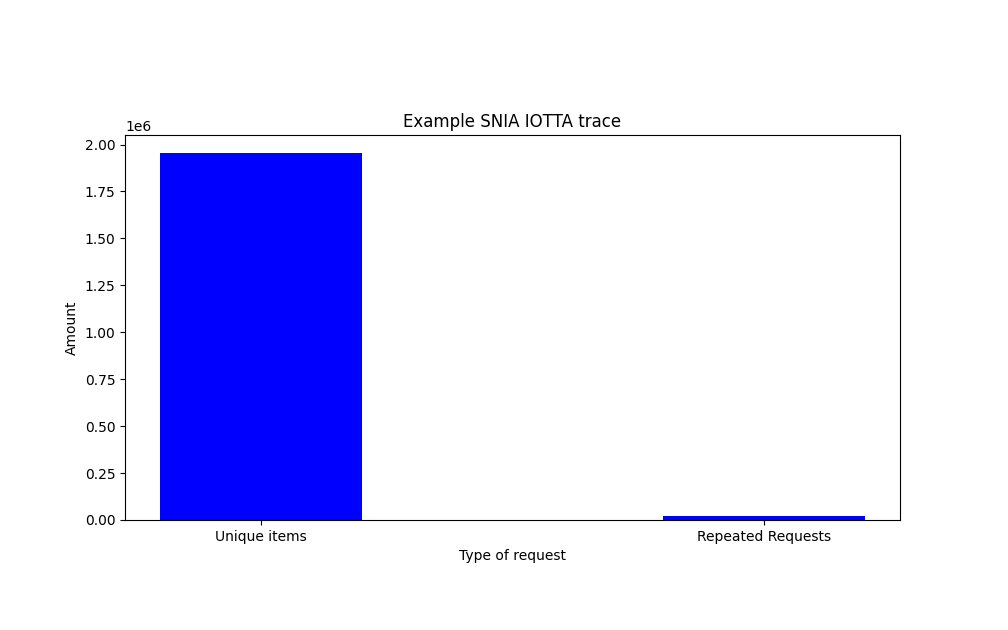
\includegraphics[scale=0.6, trim={0cm 0cm 0 0cm},clip]{thesistemplate_2020-04-24/chapters/ch5/aaaaaaaaaaaaa.png}
    \caption{Items in a SNIA IOTTA Trace}
    \label{fig:my_label}
\end{figure}


Instead of using these traces in their entirety, we instead decided to limit the number of items in a trace from \cite{snia-trace-block-io-28571}. We did this in the hope that we would get traces wherein items were accessed more frequently as there would be fewer unique items that would be accessed more frequently.

Even with this limitation, this trace generated an MRC that had the total cost paid for both Landlord and SCP so large that there was not a meaningful comparison to be made on any cache size. We then decided to not continue using these traces because of their structure. 



\subsection{Twitter Traces}
These SNIA IOTTA traces that were tested were not promising, so we sought to find traces of systems that would not suffer from the same problems of item accesses. After some searching, we found a set of traces from \cite{cacheWorkload-OSDI20} that showed some promise. Figure 5.2 shows how SCP performed versus Landlord on one of the traces provided by Twitter. As can be seen, quite clearly, these traces did not suffer the same issues as the traces from SNIA IOTTA. We chose this specific trace to show in this figure as it shows that SCP consistently pays 3\% less than Landlord on caches from size 10,000 to 100,000.


This increase in performance over Landlord was not limited to this trace though. On 82.1\% of these traces, SCP was performing within $\pm 5\%$ of Landlord. 

\begin{figure}[h]
  \begin{center}
    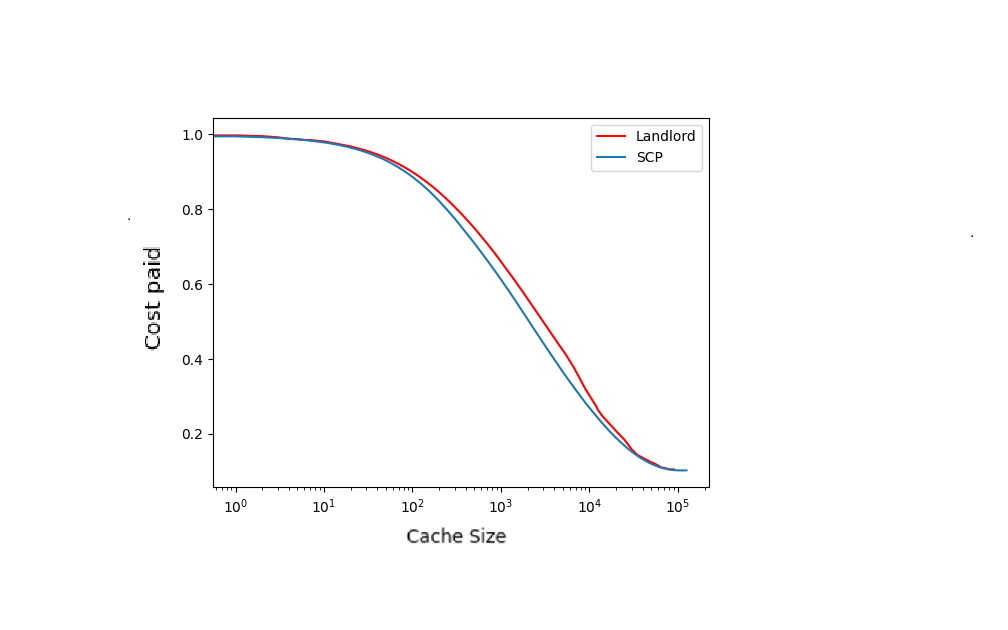
\includegraphics[scale=.5,trim={2cm 2cm 0 2cm},clip]{thesistemplate_2020-04-24/chapters/ch5/SCPresul.png}
  \end{center}
  \caption{SCPs performance vs Landlord on a Twitter trace}
\end{figure}


\subsection{Generated Traces}
With these results of the traces so far, instead of using real-world traces, we generated our own set of traces as more data points to check SCPs performance against. We generated these data to look at what happens to SCPs comparative performance to Landlord when costs either varied slightly, greatly, or not much and what happens when we vary how often items occur together.


In general, as shown in Figure 5.3, which is a sample of a generated trace, it can be seen that SCP performs almost identically to Landlord on all cache sizes. These are great results because it founds a reasonable hope that SCP will perform well as a cache algorithm in a variety of circumstances. In fact, in these traces, SCP performs $\pm 5\%$ of Landlord on $62.3\%$ of traces.


\begin{figure}[H]
    \centering
    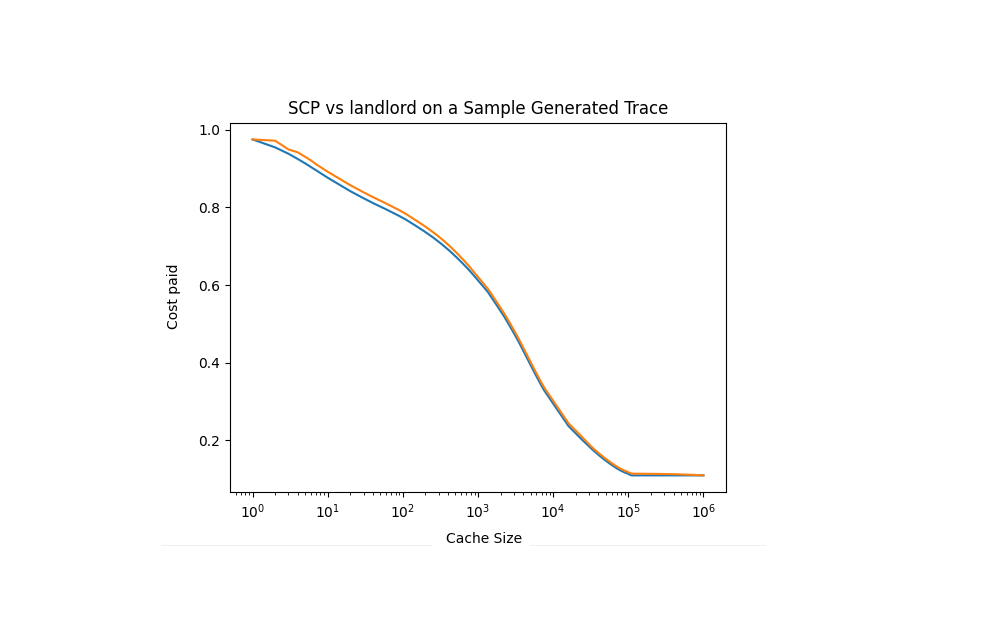
\includegraphics[scale=.6,trim={2cm 1cm 2cm 1cm},clip]{thesistemplate_2020-04-24/chapters/ch5/GenTrace.png}
    \caption{SCP's performance on a sample generated trace}
    \label{fig:my_label}
\end{figure}

\subsection{Aggregated Results}
After analyzing the traces that we gathered, both from Twitter and the generated traces, we wanted to understand how SCP performed against Landlord in total paid cost over all caches in all tested traces. This data is then shown in Figure 5.5. The positive variance is where SCP performs better than Landlord and the negative is where it performs worse. To create this graph, we normalized the cost paid on a trace to Landlord's paid cost, then found how much SCP varied from it. We did this for all cache sizes we had data for and compared them.

\begin{figure}[ht]
  \begin{center}
    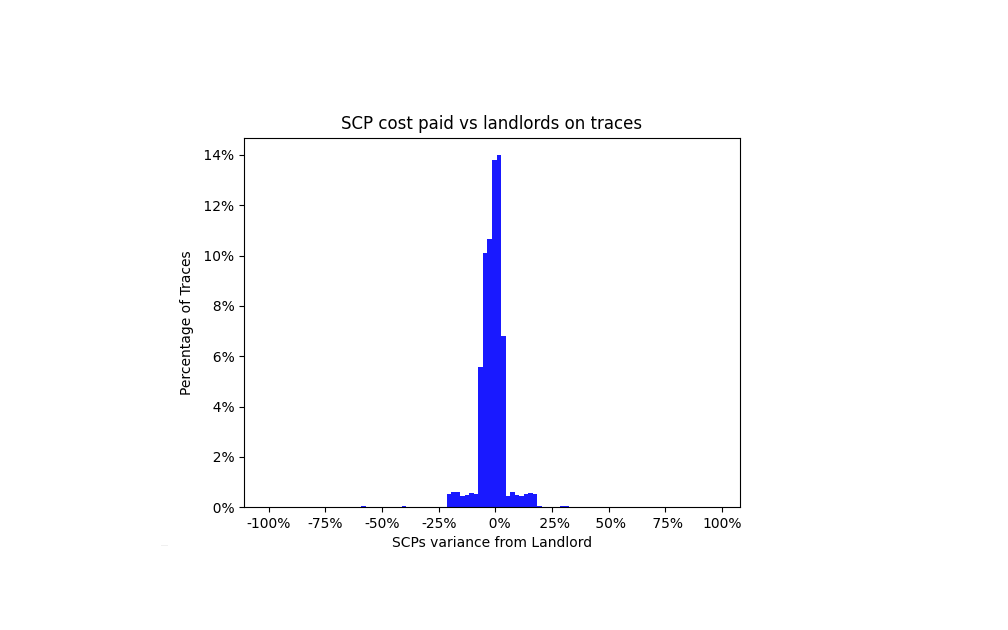
\includegraphics[scale=.6,trim={0 2cm 0 3cm},clip]{thesistemplate_2020-04-24/chapters/ch5/histFin.png}
  \end{center}
  \caption{SCP's performance over many traces}
\end{figure}


We see in Figure 5.4 that SCP performs within 5\% of Landlord 65.07\% of the time, within 25\% of landlord 99.72\% of the time, with only 0.28\% of caches performing worse than 25\%.

These results are incredibly promising and show that SCP performs well against Landlord in a variety of traces.

 

\chapter*{Conclusion}
         \addcontentsline{toc}{chapter}{Conclusion}
	\chaptermark{Conclusion}
	\markboth{Conclusion}{Conclusion}
	\setcounter{chapter}{6}
	\setcounter{section}{0}

    Caches will only become more useful as the amount of data available to computers increases over time. Up until this work, the efficient generation of MRCs was limited to the paging model and did not have a wide use case because of this limitation. This thesis introduced Sum Cost Priority (SCP), which allows for the expansion of efficient generations of MRCs to factor in cost instead of just the paging model. SCP currently has unknown theoretical performance, but the empirical results on traces when compared to Landlord are promising. We believe that this expansion of efficient MRC generation will allow more research to occur in the cost model. We also believe that it will help efficient MRC generation be expanded and generalized to more models of caching. Further research can still be done with SCP such as proving its upper competitive bound. 


%TODO TODO TODO TODO
%Spelling and grammar pass
%either leave it to be the same or discuss how we need to change it 







%If you feel it necessary to include an appendix, it goes here.
%This is where endnotes are supposed to go, if you have them.
%I have no idea how endnotes work with LaTeX.

  \backmatter % backmatter makes the index and bibliography appear properly in the t.o.c...

% if you're using bibtex, the next line forces every entry in the bibtex file to be included
% in your bibliography, regardless of whether or not you've cited it in the thesis.
    \nocite{*}

% Rename my bibliography to be called "Works Cited" and not "References" or ``Bibliography''
% \renewcommand{\bibname}{Works Cited}

%    \bibliographystyle{bsts/mla-good} % there are a variety of styles available; 
 \bibliographystyle{plainnat}
% replace ``plainnat'' with the style of choice. You can refer to files in the bsts or APA 
% subfolder, e.g. 
%\bibliographystyle{APA/apa-good}  % or
\bibliography{thesis}
 % Comment the above two lines and uncomment the next line to use biblatex-chicago.
 %\printbibliography[heading=bibintoc]

% Finally, an index would go here... but it is also optional.
\end{document}
